\chapter{Teaching with ECCE}
\label{ch:teaching}
\index{Teaching}
\index{Example sets}
\index{Central server}
\eccexample{Examples > General Chemistry}
\helppage{molecules-for-teaching}
\XXX[ chapter to be written: for teachers. The example sets by topic, the
teaching MO diagram, ECCE-QM in class, a central server for a class. The chapters
after this one are worked class demonstrations.]

\section{Atomic orbitals: radial distributions and slices}
\label{sec:atomic-orbitals}
\index{Atomic orbitals}
\index{Orbitals!atomic|see{Atomic orbitals}}
\index{Argon}
\checkedwith{9.5.3-dev}{9aa88a4ce}
\eccexample{Examples > General Chemistry > Atoms}
\helppage{density-profile}

\helppage{density-map}

The orbitals of an atom are usually drawn as boundary surfaces, a sphere for s and two lobes for p, and such a drawing hides most of what the principal quantum number does. This chapter looks at the occupied orbitals of argon in two other ways, as a curve of probability against the distance from the nucleus and as a contour map on a flat slice through the nucleus. Both views come from the same stored calculation and show the nodes, the inner maxima of 2s, 3s and 3p, and the three shells of argon.
\index{Shells}\index{Nodes}\index{Inner maxima}

\subsection{Background}
\index{Radial distribution}
\index{Radial distribution function|see{Radial distribution}}
\index{Orbitals!radial distribution|see{Radial distribution}}
\index{Probability of finding an electron|see{Radial distribution}}
An orbital $\psi(r,\theta,\phi)$ of an atom gives, through $|\psi|^2$, the probability per unit volume of finding the electron at a point. The question asked of an atom is more often how far from the nucleus the electron is, in any direction, and the answer is the radial distribution function
\begin{equation}
	P(r) = r^2 \oint |\psi(r,\theta,\phi)|^2 \, d\Omega ,
	\label{eq:rdf}
\end{equation}
the probability per unit distance of finding the electron in a thin spherical shell of radius $r$. For a normalised orbital $\int_0^\infty P(r)\,dr = 1$. For a hydrogen-like atom the orbital separates into a radial part $R_{nl}(r)$ and a spherical harmonic, and Eq.~\eqref{eq:rdf} reduces to $P(r) = r^2 R_{nl}^2(r)$. The factor $r^2$, which is the area of the sphere apart from $4\pi$, makes $P(r)$ zero at the nucleus even for an s orbital, whose density $|\psi|^2$ is largest there.

The radial part has $n-l-1$ nodes, spheres on which $\psi$ is zero and changes sign, and the orbital has $l$ angular nodes besides, planes or cones through the nucleus, so $n-1$ nodes in all.
\index{Nodes!radial}\index{Nodes!angular}\index{Nodal plane}
Between consecutive radial nodes $P(r)$ has a maximum, which gives $n-l$ maxima: one for 1s, 2p and 3d, two for 2s and 3p, three for 3s. The outermost maximum is the largest and sets the size of the orbital; the others are the inner maxima. The position of the largest maximum is the most probable radius,
\index{Most probable radius}\index{Inner maxima}
which for a hydrogen-like orbital with $l = n-1$, one without a radial node, is
\begin{equation}
	r_\mathrm{mp} = \frac{n^2 a_0}{Z},
	\label{eq:rmp}
\end{equation}
with $a_0 = \SI{0.529}{\angstrom}$ the Bohr radius and $Z$ the nuclear charge; for 1s it is $a_0/Z$.

The inner maxima are the origin of penetration.
\index{Penetration}\index{Shielding}
A 2s electron has a small maximum inside the 1s shell, close to the nucleus, where the two 1s electrons screen little of the nuclear charge, and a 2p electron has no such maximum. The 2s electron therefore feels a larger effective nuclear charge on average and lies lower in energy, which is why 2s fills before 2p and, in the next period, 3s before 3p (Section~\ref{sec:periodic-trends}). Slater's screening rules put these trends into numbers \cite{slater1930}.
\index{Effective nuclear charge}

In a many-electron atom the orbitals are no longer hydrogen-like, but the counting of nodes and maxima survives. The total electron density of argon, summed over the occupied orbitals and weighted by $r^2$, has one hump for each filled shell: 1s close to the nucleus, then 2s and 2p together, then 3s and 3p.

\subsection{What ECCE shows}
\index{Density Profile}\index{Density Map}
\index{Properties list!Density Profile}\index{Properties list!Density Map}
The Atoms topic of the General Chemistry example set holds ECCE-QM calculations of 21 atoms, H to Ar, Ca, Cr and Cu.
\index{ECCE-QM}\index{Codes!ECCE-QM}\index{Example calculations!General Chemistry}
The argon calculation uses B3LYP \cite{becke1993} with the aug-cc-pVTZ basis set \cite{woon1993}, is closed shell, and gives a total energy of $-527.490442$~hartree. Its nine occupied orbitals are 1s ($-115.118$~hartree), 2s ($-11.142$), three 2p ($-8.693$), 3s ($-0.968$) and three 3p ($-0.426$).
\index{B3LYP}\index{Basis sets!aug-cc-pVTZ}\index{Orbital energies!argon}

Two panels in the Orbitals group of the \menu{Properties} list work from the orbital coefficients and the basis set stored with the calculation. The \menu{Density Profile} plots a quantity against one length; for a single atom it opens on \menu{Around an atom}, where \menu{Radial distribution} is Eq.~\eqref{eq:rdf} evaluated for each chosen orbital and \menu{Spherical average of $\psi^2$} is the same average without the $r^2$.
\index{Density Profile!Around an atom}\index{Density Profile!Radial distribution}\index{Density Profile!Spherical average of psi2@Spherical average of $\psi^2$}
The \menu{r axis} can be \menu{Linear}, \menu{$\sqrt{r}$} or \menu{log r}; the square root spreads out the region near the nucleus, where the inner shells are, while the tick marks stay in $r$ itself.
\index{Density Profile!r axis}\index{Square-root axis}
On a $\sqrt{r}$ axis the area under a curve is no longer the number of electrons, and the panel says so beneath the plot, where the note also gives the most probable distance of each curve.
\index{Most probable radius!in the Density Profile}

The \menu{Density Map} draws one orbital, or the density, as contour lines on a flat slice. A single atom opens on \menu{This view (parallel to the screen)}, a plane through the nucleus. With \menu{Show: One orbital} the positive values are drawn as solid blue lines and the negative values as dashed vermilion lines, so that a node lies where the two colours meet; the levels start at $\pm 0.02$ and double.
\index{Density Map!One orbital}\index{Density Map!This view (parallel to the screen)}\index{Contour map}\index{Orbitals!sign|see{Phase}}\index{Phase}
The \menu{MO} box chooses the orbital, and the mouse wheel zooms the map about the pointer.

\subsection{Procedure}
\index{Opening example calculations}
\index{File menu!Open Example Calculations}
\index{Organizer!Open Example Calculations}
\index{Viewer}
\begin{enumerate}
	\item In the Organizer, choose \menu{File > Open Example Calculations}, pick \menu{General Chemistry} and click \menu{OK}. The calculations go into the project \menu{Examples}, sorted into topics.
	\item In the topic \menu{Atoms}, select the calculation \menu{Ar} and click \menu{Viewer}.
	\item In the \menu{Properties} list, click \menu{Density Profile}. The panel opens on \menu{Around an atom} with \menu{Centre} \menu{Ar1}.
	\index{Density Profile!Centre}
	\item Choose \menu{Radial distribution} and \menu{Selected orbitals}, and in the list of orbitals tick 1s, 2s and 3s and untick the others.
	\index{Density Profile!Selected orbitals}
	\item Set \menu{r axis} to \menu{$\sqrt{r}$}.
	\item To zoom, turn the mouse wheel over the plot or drag a rectangle; double-click to return to the whole plot, or click \ctrl{Show all}.
	\index{Density Profile!Show all}\index{Zooming a plot}
	\item Tick 2p, 3s and 3p instead.
	\item In the \menu{Properties} list, click \menu{Density Map} and choose \menu{Show: One orbital}.
	\item Step through the occupied orbitals 1 to 9 with the arrows of the \menu{MO} box, drawn as \ctrl{$-$} and \ctrl{+} buttons. The caption above the map names the orbital, its energy and its occupation.
	\index{Density Map!MO box}\index{Stepping through orbitals}
	\item Turn the mouse wheel over the nucleus to zoom in; double-click the map, or click \ctrl{Whole plane}, to see all of it again.
	\index{Density Map!Whole plane}\index{Zooming a map}
\end{enumerate}

\subsection{Results}
\index{Shells!of argon}
Figure~\ref{fig:ao-rdf1} shows the radial distributions of 1s, 2s and 3s on the $\sqrt{r}$ axis. 1s has a single maximum, at a most probable distance of \SI{0.0299}{\angstrom} according to the note under the plot. Equation~\eqref{eq:rmp} with $Z = 18$ gives $a_0/18 = \SI{0.0294}{\angstrom}$, and the slightly larger value is the screening of one 1s electron by the other, corresponding to an effective nuclear charge of about 17.7. 2s has one node and two maxima, the smaller at about the distance of the 1s maximum, and 3s has two nodes and three maxima, the inner two at about the distances of the 1s and 2s maxima. The number of nodes rises by one with each step in $n$. The most probable distances of 2s and 3s are \XXX[ read from the note under the plot].
\index{Effective nuclear charge}

\begin{figure}[htb]
	\centering
	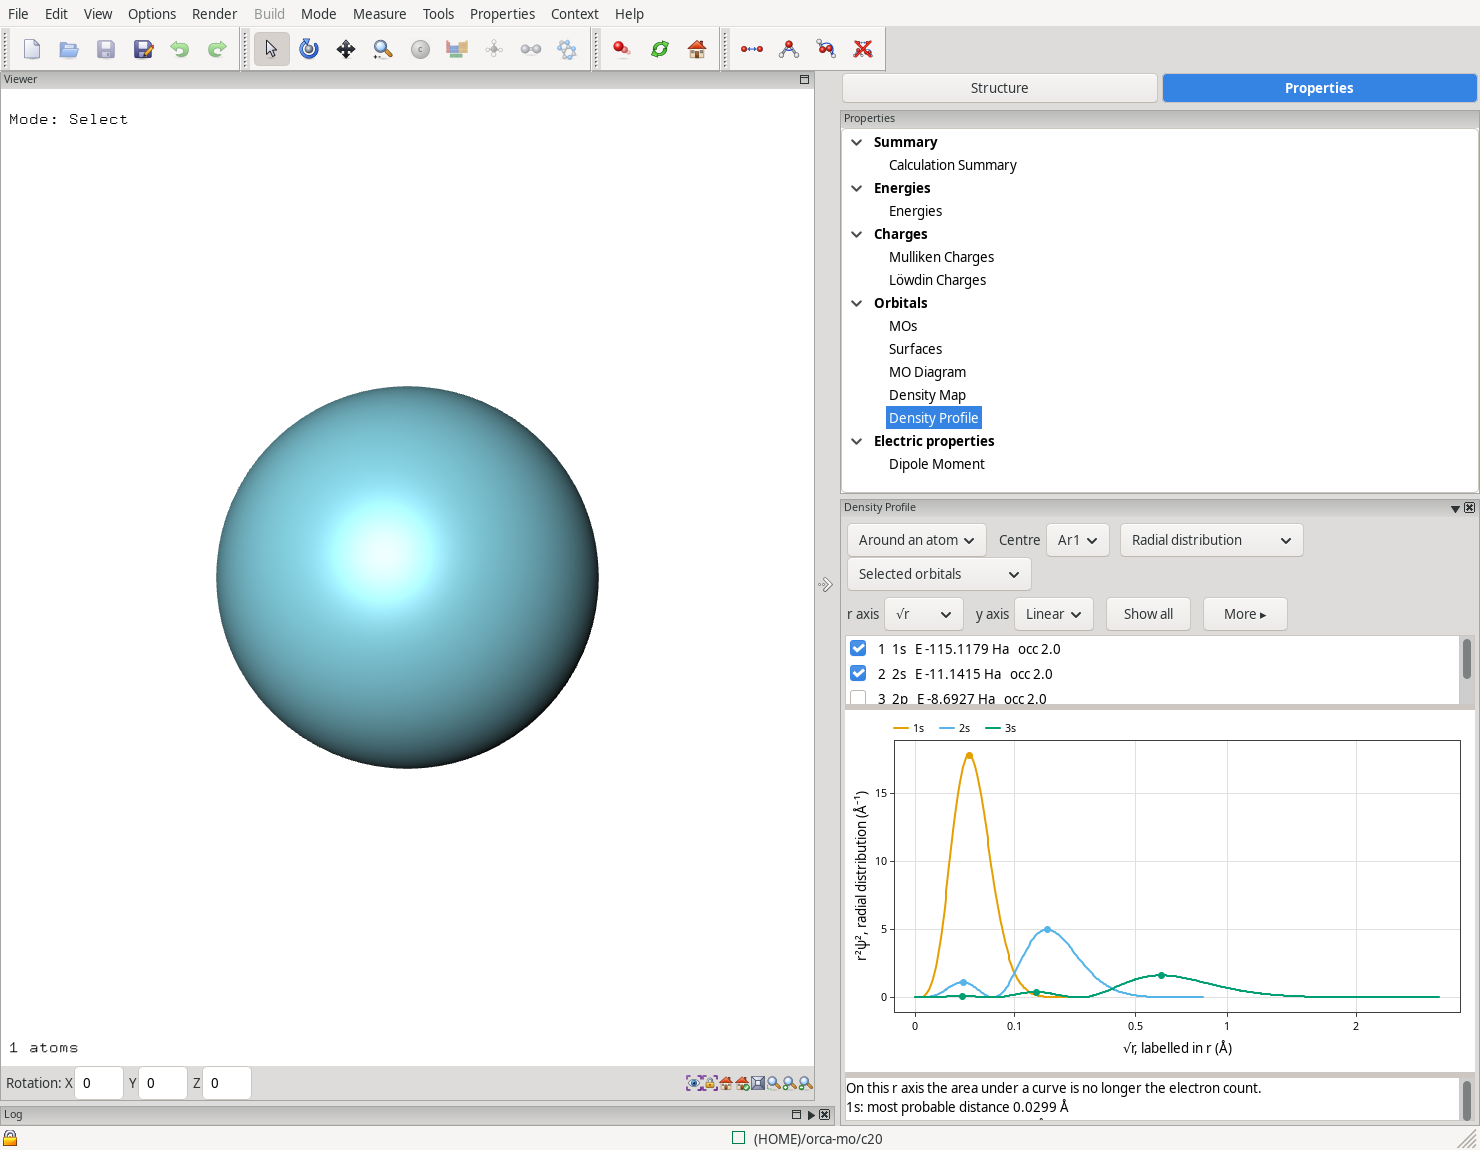
\includegraphics[width=\linewidth]{atomic-orbitals/rdf1.ecce-unknown.png}
	\caption{Argon in the Viewer, with the \menu{Density Profile} on \menu{Around an atom}, \menu{Radial distribution}, \menu{Selected orbitals} 1s, 2s and 3s and a $\sqrt{r}$ axis. \XXX[ screenshot shows a \menu{More} button where the help names \menu{Options}; regenerate from the Atoms example.]}
	\label{fig:ao-rdf1}
\end{figure}

With 2p, 3s and 3p ticked (Fig.~\ref{fig:ao-rdf2}), 2p has a single maximum and no node, and 3p has one node and two maxima. The main maxima of 3s and 3p lie at about the same distance, that of 3p slightly further out, which is what makes them one shell. Their inner maxima differ, since 3p has one, near the 2p maximum, while 3s has a second one closer still to the nucleus, at about the 1s maximum. A 3s electron therefore penetrates further than a 3p electron, and the orbital energies follow, $-0.968$~hartree for 3s against $-0.426$~hartree for 3p.
\index{Penetration!3s and 3p}

\begin{figure}[htb]
	\centering
	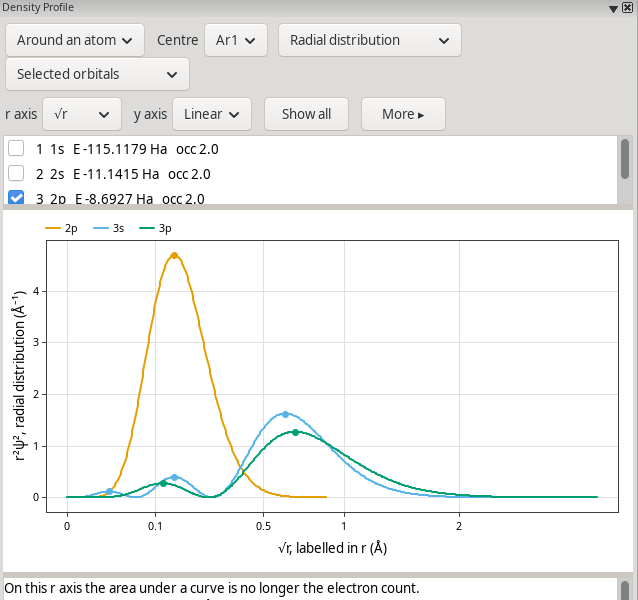
\includegraphics[width=0.75\linewidth]{atomic-orbitals/rdf2.ecce-unknown.png}
	\caption{The \menu{Density Profile} of argon with 2p, 3s and 3p ticked.}
	\label{fig:ao-rdf2}
\end{figure}

The total density of argon, with its three shells, is not among the figures yet. \XXX[ screenshot: Ar, \menu{Density Profile}, \menu{Around an atom}, \menu{Radial distribution}, \menu{Total only}, \menu{r axis} $\sqrt{r}$, showing the three humps of the total for 1s, 2s+2p and 3s+3p.]

In the \menu{Density Map} (Fig.~\ref{fig:ao-map}) orbital 6 is 3s. The circles of the contour map are the spherical nodes of the radial distribution seen edge-on. Going out from the nucleus the sign changes twice, which gives a small disc about the nucleus, a ring of opposite sign around it and the large outer part, with the sign of the disc. The disc and the ring are the two inner maxima of Fig.~\ref{fig:ao-rdf1}, and the zoomed map (Fig.~\ref{fig:ao-mapzoom}) shows how close to the nucleus they lie. The sign of 1s does not change at all, and that of 2s changes once.

\begin{figure}[htb]
	\centering
	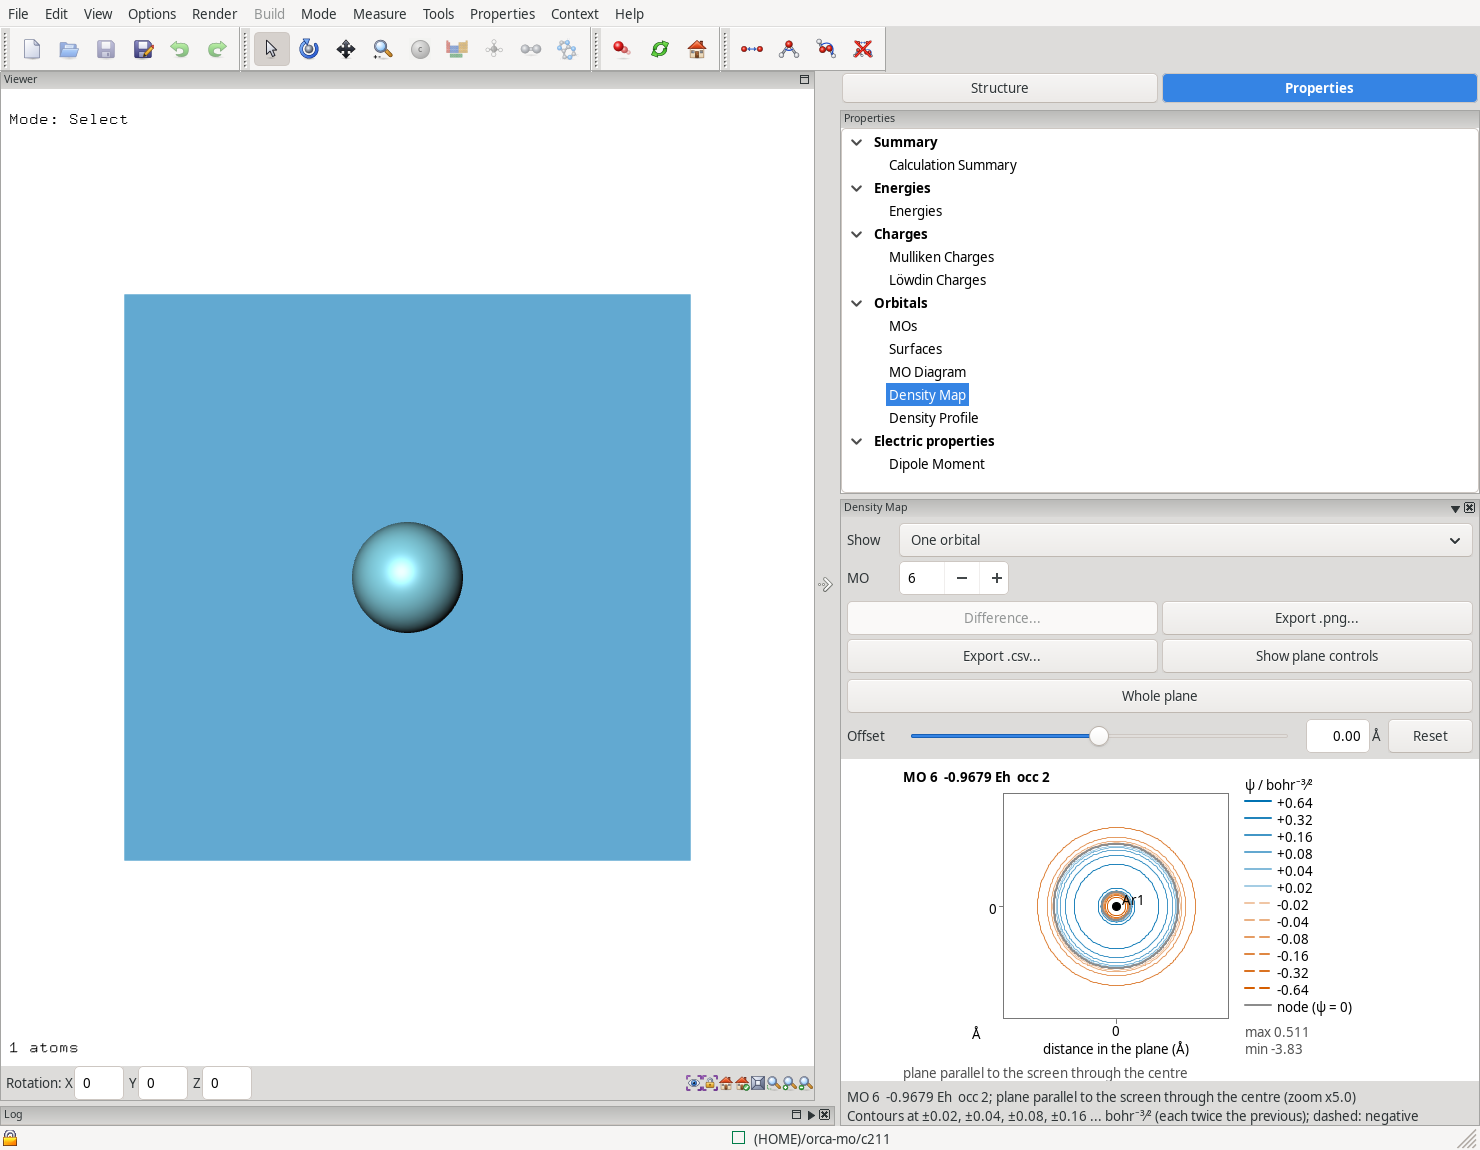
\includegraphics[width=\linewidth]{atomic-orbitals/map1.ecce-unknown.png}
	\caption{Argon with the \menu{Density Map} on \menu{One orbital}, MO 6 (3s, $-0.9679$~hartree), on the plane parallel to the screen through the nucleus; the slice is drawn in the 3-D view as a translucent square. \XXX[ screenshot shows a \menu{Show plane controls} button where the help names \menu{Options}; regenerate.]}
	\label{fig:ao-map}
\end{figure}

\begin{figure}[htb]
	\centering
	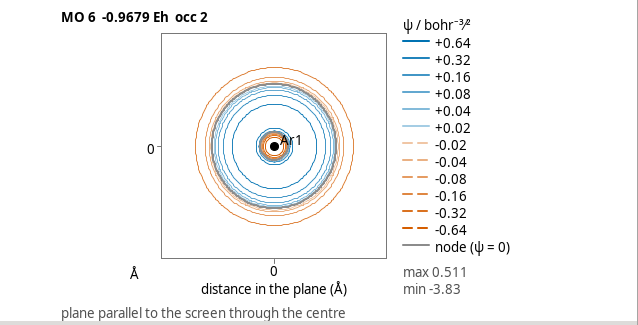
\includegraphics[width=0.75\linewidth]{atomic-orbitals/map1zoom.ecce-unknown.png}
	\caption{The map of Fig.~\ref{fig:ao-map}, zoomed in on the nucleus.}
	\label{fig:ao-mapzoom}
\end{figure}

The 2p and 3p orbitals each have a nodal plane through the nucleus, and the slice cuts the three members of each set differently: a member lying in the slice shows two lobes of opposite sign on either side of the nodal line, while one pointing out of the slice can look almost empty. \XXX[ screenshot: Ar, \menu{Density Map}, \menu{One orbital}, the member of MO 3--5 (2p) that lies in the plane, zoomed in, showing the nodal plane as a line.]
\index{Nodal plane}

\subsection{History}
Schrödinger solved the wave equation of the hydrogen atom in 1926, which gave the radial functions and their nodes \cite{schrodinger1926}, and Slater set out his rules for the screening of the nuclear charge in 1930 \cite{slater1930}.
\index{History!Schrödinger}\index{History!Slater}

\chapter{The periodic table from calculation: configurations, shielding and ionisation}
\sectionmark{The periodic table from calculation}
\label{sec:periodic-trends}
\label{sec:configurations}
\checkedwith{9.5.3-dev}{ce2531fa0}
\index{Periodic trends}
\index{Periodic table|see{Periodic trends}}
\eccexample{Examples > General Chemistry > Atoms}
\helppage{ecce-qm}

The filling order 1s, 2s, 2p, 3s, 3p, 4s, 3d is usually taught as a rule to memorise. Here we read it from calculations instead: the atoms H to Ar, Ca, Cr and Cu, and some of their ions, from the General Chemistry example set. The orbital energies give the configurations and an effective nuclear charge; total energies of atoms and ions give ionisation energies and electron affinities. The rise in ionisation energy across a period, the drop at each alkali metal and the dips at B and O all appear, and so do a few places where the numbers are easy to over-read.
\index{Electron configuration}\index{Configurations|see{Electron configuration}}
\index{Ionisation energy}\index{Ionization energy|see{Ionisation energy}}
\index{Electron affinity}

\section*{This requires}
Nothing beyond ECCE: the calculations are in the General Chemistry example set.

\section{Background}
\index{Aufbau principle}\index{Building-up principle|see{Aufbau principle}}\index{Pauli principle}
\index{Penetration}\index{Shielding}\index{Screening|see{Shielding}}\index{Subshells}
In the orbital picture, the ground state puts the electrons, two per orbital at most, into the orbitals of lowest energy. In hydrogen the energy depends on $n$ alone. In other atoms the electrons screen the nucleus from each other, and an s electron, which penetrates the inner shells, feels more of the nuclear charge than a p electron of the same shell (Chapter~\ref{sec:atomic-orbitals}). The subshells therefore separate, ns below np below nd, and for $n = 3$ and 4 enough that 4s fills before 3d.

\index{Hund's rule}\index{Multiplicity}\index{Spin multiplicity|see{Multiplicity}}
In a partly filled subshell, Hund's first rule puts the electrons in different orbitals with parallel spins. Carbon is then a triplet, nitrogen a quartet, oxygen a triplet again. Note that in a calculation the multiplicity is part of the input: you choose how many electrons are unpaired.

\index{Effective nuclear charge}\index{Zeff@$Z_\mathrm{eff}$|see{Effective nuclear charge}}
The screening can be put into one number, the effective nuclear charge $Z_\mathrm{eff} = Z - S$, where $Z$ is the nuclear charge and $S$ the screening constant. Slater's rules estimate $S$ from the configuration \cite{slater1930}. For an electron in an s or p orbital of shell $n$, every other electron in the same shell contributes 0.35 to $S$ (0.30 within 1s), every electron in shell $n-1$ contributes 0.85, and every electron further in contributes 1.00. For the 2s electron of lithium, $1s^2 2s^1$, the two 1s electrons give $S = 2 \times 0.85 = 1.70$, so that $Z_\mathrm{eff} = 3 - 1.70 = 1.30$. For a 2p electron of neon, $1s^2 2s^2 2p^6$, the seven other $n = 2$ electrons and the two 1s electrons give $S = 7 \times 0.35 + 2 \times 0.85 = 4.15$ and $Z_\mathrm{eff} = 10 - 4.15 = 5.85$.

A second estimate comes from the calculation itself. It treats an orbital of energy $\varepsilon$ as if it were a hydrogen-like orbital of the same $n$, for which $\varepsilon = -Z^2/2n^2$ in hartree, and solves for the charge:
\begin{equation}
	\varepsilon = -\frac{Z_\mathrm{eff}^2}{2n^2}\ \text{hartree}, \qquad
	Z_\mathrm{eff} = n\sqrt{-2\varepsilon/\text{hartree}} .
	\label{eq:zeff}
\end{equation}
The two are not the same thing. An orbital energy contains the repulsion with every other electron, including those of the same shell, and equation~\eqref{eq:zeff} puts all of it into $Z_\mathrm{eff}$.

\index{Koopmans' theorem}\index{Ionisation energy!from orbital energies}\index{Delta SCF@$\Delta$SCF}\index{Relaxation}\index{Electron correlation}\index{HOMO}
The first ionisation energy is $\mathrm{IE} = E(\mathrm{A}^+) - E(\mathrm{A})$, the electron affinity $\mathrm{EA} = E(\mathrm{A}) - E(\mathrm{A}^-)$, positive when the anion is more stable. Both come from two total energies (the $\Delta$SCF route). Koopmans' theorem gives a shortcut for Hartree-Fock: $\mathrm{IE} \approx -\varepsilon_\mathrm{HOMO}$, where HOMO is the highest occupied orbital, if the other orbitals do not change \cite{koopmans1934}. Two errors enter. The remaining electrons relax towards the hole, which makes $-\varepsilon_\mathrm{HOMO}$ too large. Hartree-Fock also leaves out electron correlation, the part of the repulsion between electrons that its average field misses because the electrons in fact avoid each other; the correlation energy is larger in the atom than in the cation and makes the Hartree-Fock IE too small. $\Delta$SCF includes the relaxation but not the correlation. For a density functional such as B3LYP, $-\varepsilon_\mathrm{HOMO}$ is well below the IE.

ECCE gives orbital energies in hartree and the Energy Calculator gives energy differences in kJ/mol, kcal/mol and eV. The conversions used in this chapter are 1~hartree = 27.2114~eV = 2625.50~kJ/mol.

\section{The calculations}
\index{ECCE-QM}\index{Codes!ECCE-QM}\index{Example calculations!General Chemistry}
\index{B3LYP}\index{Basis sets!aug-cc-pVTZ}\index{Basis sets!def2-TZVPD}\index{Basis sets!cc-pVTZ}\index{ROKS}\index{Restricted open shell}
\index{Hartree-Fock}\index{UHF}\index{PBE0}\index{Basis sets!aug-cc-pVDZ}
Three topics of the General Chemistry example set hold the ECCE-QM calculations:
\begin{enumerate}
	\item \menu{Atoms}: the 21 atoms, B3LYP \cite{becke1993}, aug-cc-pVTZ \cite{kendall1992,woon1993} for H to Ar, cc-pVTZ for Ca, def2-TZVPD \cite{rappoport2010} for Cr and Cu. Closed shells are restricted, open shells restricted open-shell (ROKS): the alpha and beta electrons share one set of spatial orbitals. The aug-cc-pVTZ basis is of triple-zeta quality with diffuse functions, which describe the loosely bound outer electrons; cc-pVTZ lacks the diffuse functions, and def2-TZVPD is a triple-zeta basis with diffuse functions from another family.
	\item \menu{Koopmans' theorem}: H to Ar, Hartree-Fock/aug-cc-pVTZ, unrestricted (UHF) for open shells, so that the alpha and beta electrons have orbitals, and orbital energies, of their own.
	\item \menu{Ionisation energies and electron affinities}: Li, Be, C, N, O, F, Ne and their cations (Hartree-Fock/aug-cc-pVTZ); Li, Be, C, N, O, F and their anions (PBE0/aug-cc-pVDZ \cite{adamo1999}).
\end{enumerate}
Each calculation has a note saying what it shows.

\index{MOs panel}\index{Properties list!MOs}\index{MOs panel!Compute}\index{MO Diagram}\index{Properties list!MO Diagram}\index{Orbital energies}
In the Viewer, the \menu{MOs} panel lists the orbitals with their energy and occupation. Select a row and click \ctrl{Compute} to draw the orbital, which tells s from p or d. \menu{Tools > Energy Calculator...} in the Organizer takes two calculations, A then B, and gives \menu{B - A} in kJ/mol, kcal/mol and eV.
\index{Energy Calculator}\index{Tools menu!Energy Calculator...}\index{Energy Calculator!B - A}
\index{Calculating an ionisation energy}\index{Calculating an electron affinity}
\helppage{energy-calculator}

\section{Procedure}
\index{Opening example calculations}\index{File menu!Open Example Calculations}\index{Organizer!Open Example Calculations}\index{Viewer}
\begin{enumerate}
	\item In the Organizer, choose \menu{File > Open Example Calculations}, pick \menu{General Chemistry} and click \menu{OK}.
	\item In \menu{Atoms}, select \menu{Ne}, click \menu{Viewer} and open \menu{MOs}. Read the energies of 1s, 2s and 2p.
	\item Select \menu{Na}, \menu{C}, \menu{N} and \menu{O} in turn. Count the singly occupied orbitals (\menu{Occ \#} 1) and compare with the multiplicity.
	\item Select \menu{Ca}, \menu{Cr} and \menu{Cu}. Find 4s and 3d near the top of the occupied list; \ctrl{Compute} tells which is which.
	\item In \menu{Koopmans' theorem}, open \menu{N\_HF} and \menu{O\_HF} and read the energy of the highest occupied orbital. The \menu{MOs} panel lists the alpha orbitals first and the beta orbitals below them; in an open shell the highest occupied orbital can be a beta one, as in oxygen, so compare the last occupied orbital of each set. Multiply by $-27.2114$ to get the Koopmans IE in eV.
	\index{Koopmans' theorem!in the MOs panel}
	\item In \menu{Koopmans' theorem}, open \menu{Li\_HF}, read \menu{E (Hartree)} of the highest occupied orbital (\menu{Occ \#} 1, the 2s) and calculate $Z_\mathrm{eff} = n\sqrt{-2\varepsilon}$ with $n = 2$ (equation~\eqref{eq:zeff}). Repeat for \menu{Ne\_HF} and \menu{Na\_HF} ($n = 3$), and compare with Slater's rules.
	\index{Effective nuclear charge!calculating}
	\item In \menu{Ionisation energies and electron affinities}, select \menu{N\_HF\_neutral}, Ctrl-click \menu{N\_HF\_cation} and choose \menu{Tools > Energy Calculator...}. \menu{B - A} is the ionisation energy. Repeat for the other pairs.
	\item For an electron affinity, select the anion first (\menu{F\_anion}), then the atom (\menu{F\_PBE0\_neutral}). \menu{B - A} is the electron affinity.
\end{enumerate}

\section{Configurations}
\index{Electron configuration!of the atoms H to Ar}\index{Orbital energies!of the atoms}\index{Penetration!2s and 2p}\index{Neon}\index{Sodium}
Every atom fills its orbitals in the Aufbau order (table~\ref{tab:pt-config}). Neon shows the split of a shell most clearly: 2s at $-1.459$ and 2p at $-0.572$~hartree, 24~eV apart although both have $n = 2$. In sodium the next electron goes into 3s at $-0.125$~hartree, and the 2p has dropped to $-1.156$~hartree, into the core.

\begin{table}[htb]
	\centering\small
	\caption{Atoms H to Ar (B3LYP/aug-cc-pVTZ): multiplicity used, valence configuration and valence orbital energies in hartree. Where singly and doubly occupied p orbitals differ in energy, both are given, singly occupied first.}
	\label{tab:pt-config}
	\begin{tabular}{lcl rr}
		\hline
		Atom & $2S+1$ & Valence configuration & $\varepsilon(n\mathrm{s})$ & $\varepsilon(n\mathrm{p})$ \\
		\hline
		H  & 2 & 1s$^1$         & $-0.319$ & \\
		He & 1 & 1s$^2$         & $-0.658$ & \\
		Li & 2 & 2s$^1$         & $-0.131$ & \\
		Be & 1 & 2s$^2$         & $-0.229$ & \\
		B  & 2 & 2s$^2$2p$^1$   & $-0.371$ & $-0.185$ \\
		C  & 3 & 2s$^2$2p$^2$   & $-0.533$ & $-0.265$ \\
		N  & 4 & 2s$^2$2p$^3$   & $-0.713$ & $-0.355$ \\
		O  & 3 & 2s$^2$2p$^4$   & $-0.942$ & $-0.460$ / $-0.362$ \\
		F  & 2 & 2s$^2$2p$^5$   & $-1.191$ & $-0.565$ / $-0.464$ \\
		Ne & 1 & 2s$^2$2p$^6$   & $-1.459$ & $-0.572$ \\
		Na & 2 & 3s$^1$         & $-0.125$ & \\
		Mg & 1 & 3s$^2$         & $-0.192$ & \\
		Al & 2 & 3s$^2$3p$^1$   & $-0.306$ & $-0.129$ \\
		Si & 3 & 3s$^2$3p$^2$   & $-0.421$ & $-0.191$ \\
		P  & 4 & 3s$^2$3p$^3$   & $-0.540$ & $-0.259$ \\
		S  & 3 & 3s$^2$3p$^4$   & $-0.678$ & $-0.333$ / $-0.274$ \\
		Cl & 2 & 3s$^2$3p$^5$   & $-0.821$ & $-0.407$ / $-0.348$ \\
		Ar & 1 & 3s$^2$3p$^6$   & $-0.968$ & $-0.426$ \\
		\hline
	\end{tabular}
\end{table}

\index{Hund's rule!carbon, nitrogen and oxygen}\index{Carbon}\index{Nitrogen}\index{Oxygen}\index{S2@$S^2$ expectation value}
Carbon has two singly occupied 2p orbitals and the third empty, nitrogen three singly occupied, oxygen one doubly and two singly occupied. These are Hund's arrangements, but be clear with students where they come from: the multiplicity was set in the input. The topic has no singlet carbon or doublet nitrogen, so it does not show that high spin is lower; for that you need a second calculation of the same atom. The expectation value $\langle S^2 \rangle$, under \menu{Properties > Summary > S**2}, confirms the spin state asked for, since $\langle S^2 \rangle = S(S+1)$: 2.000 for the triplets, 3.750 for the quartets, 12.000 for chromium.

\index{Restricted open shell!orbital energies}
Watch out with O, F, S and Cl. In the restricted open-shell calculation the singly occupied 2p orbitals of oxygen lie at $-0.460$~hartree, \emph{below} the doubly occupied one at $-0.362$. This comes from how restricted open-shell orbital energies are defined; it does not mean the unpaired electrons are bound more strongly. The unrestricted Hartree-Fock orbitals show the physics more directly (section~\ref{sec:pt-dips}).

\section{4s and 3d: calcium, chromium and copper}
\index{4s and 3d}\index{3d and 4s|see{4s and 3d}}\index{Calcium}\index{Chromium}\index{Copper}
\index{Chromium!3d5 4s1@3d$^5$4s$^1$}\index{Copper!3d10 4s1@3d$^{10}$4s$^1$}
The \menu{MO Diagram} panel (\menu{Properties > Orbitals > MO Diagram}, with \ctrl{Energies to scale} ticked) gives each level in eV and draws the electrons as arrows; figure~\ref{fig:pt-tm} shows it for copper. In calcium the two outer electrons are in 4s ($-4.11$~eV). Chromium (septet, 3d$^5$4s$^1$) has its 3d at $-4.93$~eV and 4s at $-4.65$~eV; copper (doublet, 3d$^{10}$4s$^1$) has 3d at $-6.90$~eV and 4s at $-5.24$~eV. Across the series 3d falls below 4s, so 4s is the highest occupied orbital and is lost first, which is why Cr$^+$ and Cu$^+$ keep their 3d$^5$ and 3d$^{10}$ cores.

\begin{figure}[htbp]
	\centering
	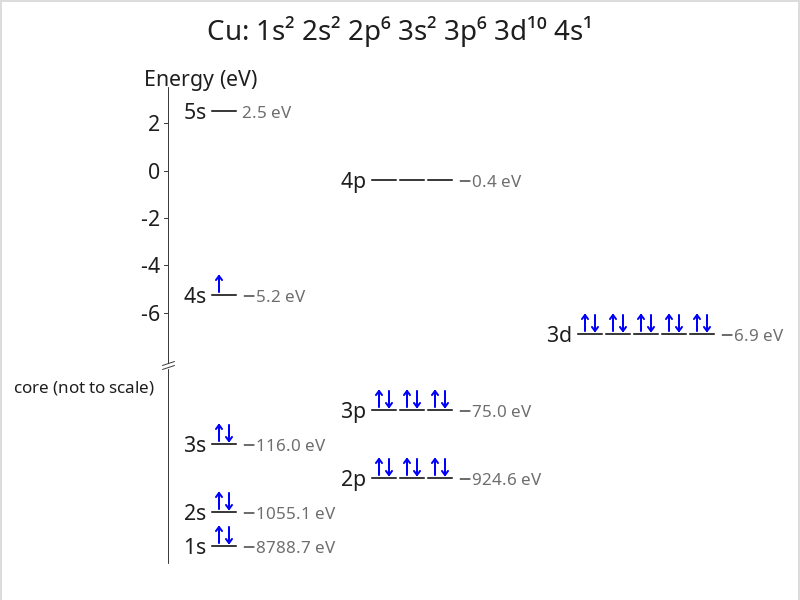
\includegraphics[width=0.8\linewidth]{periodic-trends/tm-mo-cu.ecce-9.5.3-dev.png}
	\caption{The \menu{MO Diagram} panel of copper (B3LYP), energies to scale, with the core below the axis break. The filled 3d level lies below the singly occupied 4s.}
	\label{fig:pt-tm}
\end{figure}

Do not teach the exceptions from this figure. Orbital energies do not decide the configuration; total energies do, and 3d$^4$4s$^2$ chromium or 3d$^9$4s$^2$ copper would each be a separate calculation. The topic has only the observed configurations, so it cannot show that they are the lower ones. The empty orbitals of calcium depend on the basis set, so their order is not to be taught either. \XXX[ check whether ECCE-QM can hold copper in 3d$^9$4s$^2$.]
\index{Exceptions to the Aufbau order}\index{Aufbau principle!exceptions}

\section{Effective nuclear charge}
\index{Effective nuclear charge!from orbital energies}
We take the energy of the highest occupied orbital from the \menu{MOs} panel of the Hartree-Fock calculations in \menu{Koopmans' theorem}, where the column \menu{E (Hartree)} gives it in the unit that equation~\eqref{eq:zeff} needs. For lithium the 2s orbital of \menu{Li\_HF} lies at $-0.1964$~hartree, so that
\begin{equation*}
	Z_\mathrm{eff} = 2\sqrt{2 \times 0.1964} = 2\sqrt{0.3928} = 1.25 ,
\end{equation*}
and for neon the 2p orbitals of \menu{Ne\_HF} lie at $-0.8512$~hartree, which gives $Z_\mathrm{eff} = 2\sqrt{1.7024} = 2.61$. For the third period $n = 3$: the 3s orbital of sodium at $-0.1822$~hartree gives $3\sqrt{0.3644} = 1.81$. Figure~\ref{fig:pt-zeff} shows the same calculation for every atom from H to Ar. Across a period it rises by about 0.3 per element, from 1.25 (Li) to 2.61 (Ne) and from 1.81 (Na) to 3.26 (Ar), because each added proton is only partly screened by the electron added with it. It falls back at each alkali metal, where a new shell starts. The breaks at B, Al, O and S are the same as in the ionisation energies, since this $Z_\mathrm{eff}$ is the Koopmans IE in other units.

\begin{figure}[htbp]
	\centering
	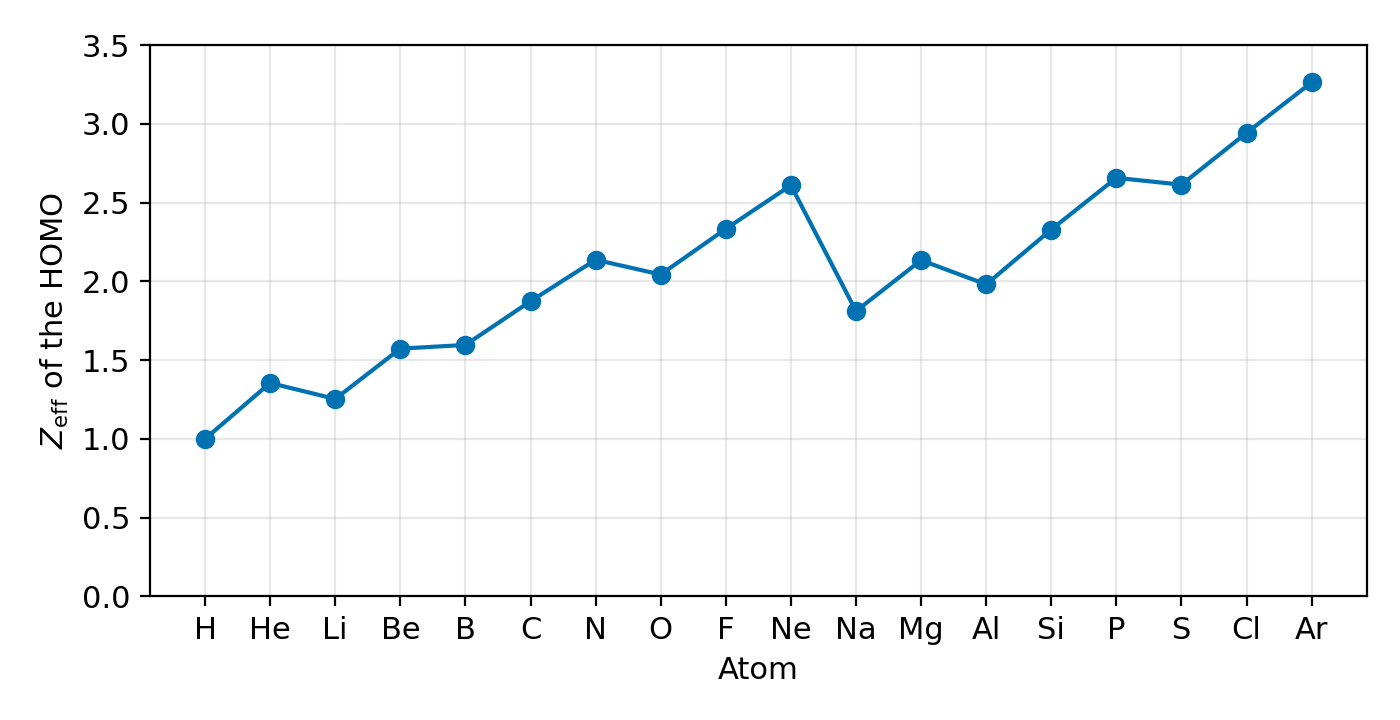
\includegraphics[width=0.85\linewidth]{periodic-trends/zeff.ecce-9.5.2-dev.png}
	\caption{Effective nuclear charge of the highest occupied orbital from equation~\eqref{eq:zeff} and Hartree-Fock/aug-cc-pVTZ orbital energies, plotted from the values in the \menu{MOs} panel.}
	\label{fig:pt-zeff}
\end{figure}

\index{Slater's rules}
For one electron outside a closed shell the estimate agrees with Slater's rules: 1.25 against 1.30 for lithium. For a full shell it does not: Slater gives 5.85 for the 2p of neon, equation~\eqref{eq:zeff} 2.61. The difference is the repulsion with the other seven $n = 2$ electrons, which the orbital energy contains. Teach the trend across a period; the absolute values depend on the definition.

\section{First ionisation energies}
\index{Ionisation energy!across a period}\index{Periodic trends!ionisation energy}\index{Comparing with experiment}
Table~\ref{tab:pt-ie} and figure~\ref{fig:pt-ie} compare the calculated values with experiment \cite{nistasd}. Koopmans' values show the whole textbook curve: the rise across a period, the maxima at the noble gases, the drops to Li and Na, the dips at O, S and Al. Hydrogen gives 13.60~eV, as it must for one electron.

\begin{table}[htb]
	\centering\small
	\caption{First ionisation energies in eV. Koopmans: $-\varepsilon_\mathrm{HOMO}$, Hartree-Fock/aug-cc-pVTZ. $\Delta$SCF: $E(\mathrm{A}^+) - E(\mathrm{A})$, Hartree-Fock/aug-cc-pVTZ. B3LYP: $-\varepsilon_\mathrm{HOMO}$. Experiment: NIST ASD \cite{nistasd}.}
	\label{tab:pt-ie}
	\begin{tabular}{l rrrr}
		\hline
		Atom & Koopmans & $\Delta$SCF & B3LYP & Experiment \\
		\hline
		H  & 13.60 &       &  8.68 & 13.60 \\
		He & 24.98 &       & 17.90 & 24.59 \\
		Li &  5.34 &  5.34 &  3.57 &  5.39 \\
		Be &  8.42 &  8.04 &  6.24 &  9.32 \\
		B  &  8.67 &       &  5.03 &  8.30 \\
		C  & 11.94 & 10.80 &  7.22 & 11.26 \\
		N  & 15.53 & 13.90 &  9.67 & 14.53 \\
		O  & 14.20 & 12.03 &  9.85 & 13.62 \\
		F  & 18.51 & 15.67 & 12.63 & 17.42 \\
		Ne & 23.16 & 19.69 & 15.57 & 21.56 \\
		Na &  4.96 &       &  3.41 &  5.14 \\
		Mg &  6.89 &       &  5.21 &  7.65 \\
		Al &  5.93 &       &  3.51 &  5.99 \\
		Si &  8.20 &       &  5.19 &  8.15 \\
		P  & 10.67 &       &  7.04 & 10.49 \\
		S  & 10.32 &       &  7.46 & 10.36 \\
		Cl & 13.09 &       &  9.47 & 12.97 \\
		Ar & 16.09 &       & 11.59 & 15.76 \\
		\hline
	\end{tabular}
\end{table}

\begin{figure}[htbp]
	\centering
	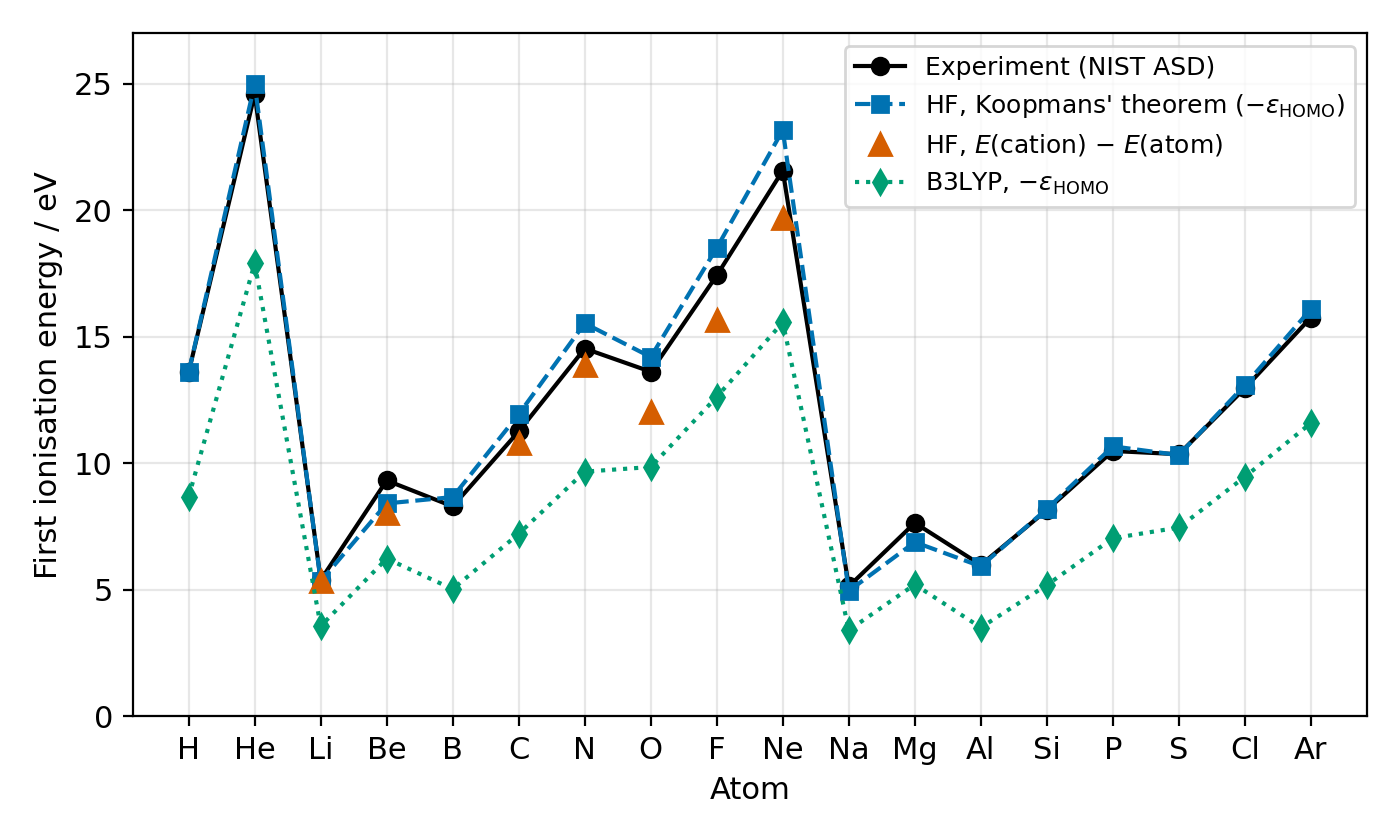
\includegraphics[width=\linewidth]{periodic-trends/ie.ecce-9.5.2-dev.png}
	\caption{First ionisation energies of H to Ar. Black: experiment \cite{nistasd}. Blue: Koopmans. Orange: $\Delta$SCF. Green: $-\varepsilon_\mathrm{HOMO}$ from B3LYP.}
	\label{fig:pt-ie}
\end{figure}

\index{Koopmans' theorem!errors}\index{Relaxation}
$\Delta$SCF is below experiment for all seven atoms, by 0.05~eV at Li and 1.6 to 1.9~eV at O, F and Ne: the missing correlation. Koopmans' values lie above $\Delta$SCF by the relaxation energy (1.1~eV for C, 3.5~eV for Ne). The two errors partly cancel, which is why Koopmans' theorem looks good in figure~\ref{fig:pt-ie}. Do not present it as the more accurate method. For lithium the relaxation is negligible: the Koopmans value, $0.1964~\text{hartree} = 5.344$~eV, and $\Delta$SCF, 5.342~eV from the Energy Calculator, agree to 0.002~eV, because removing the outer electron hardly changes the core.

\index{B3LYP!orbital energies}\index{Density functional theory!HOMO energy}
The B3LYP orbital energies follow the same pattern a few eV lower (8.68~eV for hydrogen). With a density functional, take ionisation energies from total energies, not orbital energies.

\section{The dips at boron and oxygen}
\label{sec:pt-dips}
\index{Ionisation energy!dip at boron}\index{Ionisation energy!dip at oxygen}\index{Boron}\index{Aluminium}\index{Sulfur}
The measured IE falls from Be to B, from N to O, and again from Mg to Al and from P to S. At B and Al the electron removed is the first p electron, which penetrates less than an s electron. At O and S it is the first electron to pair in a p orbital.

\index{Pairing energy}\index{Electron pairing}
The unrestricted Hartree-Fock calculations show the pairing directly. In nitrogen the three alpha 2p orbitals lie at $-0.571$~hartree and there is no beta 2p electron. In oxygen the fourth 2p electron is beta, paired in an orbital with an alpha electron, and lies at $-0.522$~hartree, above all the alpha 2p orbitals. Koopmans gives 14.20~eV for oxygen against 15.53~eV for nitrogen. $\Delta$SCF drops by 1.87~eV, twice the measured 0.92~eV (from the unrounded values 14.534 and 13.618~eV), since Hartree-Fock misses more correlation in oxygen, which has one more electron pair. The cations confirm the counts: O$^+$ is a quartet, N$^+$ a triplet.

\index{Koopmans' theorem!failure for beryllium}\index{Beryllium}
At boron Koopmans' theorem fails: its values \emph{rise} from Be to B (8.42 to 8.67~eV) where experiment falls. Beryllium is 0.90~eV too low, because its 2s$^2$ pair mixes strongly with the nearby empty 2p, a correlation Hartree-Fock omits. Between Mg and Al the gap is wide enough that Koopmans' values fall (6.89 to 5.93~eV). Show the s-to-p dip in the third period.

\section{Electron affinities}
\index{Electron affinity!across a period}\index{Anions}
Table~\ref{tab:pt-ea} gives the electron affinities from PBE0/aug-cc-pVDZ. Fluorine takes up an electron most readily (3.29~eV), filling its 2p. Carbon and oxygen give about 1.4~eV, lithium 0.49~eV. Beryllium and nitrogen come out negative: the anion is higher than the atom. In beryllium the new electron has to go into 2p; in nitrogen it has to pair. These are the same two effects as in the IE dips.

\begin{table}[htb]
	\centering\small
	\caption{Electron affinities, $E(\mathrm{A}) - E(\mathrm{A}^-)$, PBE0/aug-cc-pVDZ, with the multiplicities of atom and anion.}
	\label{tab:pt-ea}
	\begin{tabular}{l cc rr r}
		\hline
		Atom & $2S+1$ atom & $2S+1$ anion & EA / eV & EA / kJ\,mol$^{-1}$ & Experiment / eV \\
		\hline
		Li & 2 & 1 &  0.49 &  47.4 & \XXX \\
		Be & 1 & 2 & $-0.04$ & $-3.8$ & \XXX \\
		C  & 3 & 4 &  1.41 & 136.5 & \XXX \\
		N  & 4 & 3 & $-0.12$ & $-11.7$ & \XXX \\
		O  & 3 & 2 &  1.39 & 134.5 & \XXX \\
		F  & 2 & 1 &  3.29 & 317.6 & \XXX \\
		\hline
	\end{tabular}
\end{table}

\index{Electron affinity!negative}
A negative EA in a finite basis set is only an indication: an unbound anion has no stable state, and its computed energy depends on the basis set. Teach the sign, not the size. Never read an EA from the anion's orbital energies: the HOMO of Li$^-$ and C$^-$ lies above zero, although both anions are bound by total energy.

\section{History}
\index{History!Koopmans}\index{History!Slater}\index{History!Hund}
Slater published his screening rules in 1930 \cite{slater1930}, Koopmans his theorem in 1934 \cite{koopmans1934}. Hund's rules came from his analysis of atomic spectra \XXX[ citation and year].

\chapter{Polar covalent and ionic bonds}
\label{ch:t-polar-ionic}
\index{Polar bond}
\index{Ionic bond}
\index{Dipole moment}
\index{Localised orbitals}
\eccexample{Examples > General Chemistry > Polar bonds and dipole moments}

A textbook draws \chem{H2} with a shared electron pair, \chem{NaCl} as two ions and \chem{HF} somewhere in between, and students ask where the line between a covalent and an ionic bond lies. This chapter gives the teacher one number for each of six molecules that answers the question on the board: how much charge has moved from one atom to the other, worked out from the dipole moment and the bond length. The numbers show that the charge separation grows step by step from \chem{HBr} to \chem{NaCl}, with no jump, and the localised orbitals of \chem{HF} and \chem{LiF} show where a chemist stops drawing a bond between the two atoms.

\section*{This requires}
Nothing beyond ECCE: the calculations are in the General Chemistry example set.

\section{The calculations}
Six stored calculations of single molecules in the gas phase are used. \emph{HF\_dipole}, \emph{HCl} and \emph{HBr} are in the topic \menu{Polar bonds and dipole moments}, \emph{LiH} and \emph{LiF} in \menu{Molecular orbitals of diatomics}, and \emph{nacl\_ion\_pair} in \menu{Intermolecular interactions}. Each is an optimised structure, so the bond length is the one the calculation finds for the molecule at rest.
\XXX[LiF: the stored optimisation stopped after 100 steps without meeting its convergence criteria (bond length steady at 1.554~\AA, no frequencies). Rerun before release; the numbers below are from the last step.]

\section{Procedure}
\begin{enumerate}
	\item In the Organizer, choose \menu{File > Open Example Calculations}, pick \menu{General Chemistry} and click \menu{OK}.
	\item Open \emph{HF\_dipole} in the Viewer. With \menu{Measure} (Chapter~\ref{ch:first-calculation}), measure the H--F distance.
	\item Open \menu{Properties > Electric properties > Dipole Moment} and read the total dipole moment in debye.
	\item Repeat for \emph{HCl}, \emph{HBr}, \emph{LiH}, \emph{LiF} and \emph{nacl\_ion\_pair}.
	\item In \emph{HF\_dipole} and \emph{LiF}, open \menu{Properties > Orbitals > MOs}, choose \menu{Localised MO} in the box next to \menu{Compute}, and read the \menu{Bond type} column.
\end{enumerate}
\index{Dipole moment!showing}

\section{How much charge has moved}
A dipole moment $\mu$ is a charge $q$ times the distance $R$ that separates it from an equal and opposite charge, $\mu = qR$. If one whole electron had moved from one atom to the other, the dipole moment would be $eR$; with $R$ in \AA{} and $\mu$ in debye (D, the unit in which dipole moments are tabulated) that is $4.803\,R$~D. Dividing the dipole moment by this value gives the fraction of an electron that has moved, $q/e = \mu/(4.803\,R)$: 0 for a bond shared equally, 1 for two whole ions. This number needs only the dipole moment and the bond length, and both can be measured, so calculation and experiment can be put side by side (table~\ref{tab:pi-q}).

\begin{table}[htbp]
	\centering
	\caption{Bond length $R$, dipole moment $\mu$ and the fraction of an electron moved, $q/e=\mu/(4.803\,R)$, for six molecules in the gas phase. Calculated values from the stored ECCE calculations; measured bond lengths from the NIST Chemistry WebBook \cite{nistwebbook}, measured dipole moments from the NIST CCCBDB \cite{cccbdb}.}
	\label{tab:pi-q}
	\begin{tabular}{lrrrrrr}
		\toprule
		& \multicolumn{3}{c}{calculated} & \multicolumn{3}{c}{measured} \\
		\cmidrule(lr){2-4}\cmidrule(lr){5-7}
		Molecule & $R$ (\AA) & $\mu$ (D) & $q/e$ & $R$ (\AA) & $\mu$ (D) & $q/e$ \\
		\midrule
		\chem{HBr}  & 1.428 & 1.01 & 0.15 &       & 0.83 & \\
		\chem{HCl}  & 1.290 & 1.47 & 0.24 &       & 1.09 & \\
		\chem{HF}   & 0.935 & 1.86 & 0.42 & 0.917 & 1.83 & 0.42 \\
		\chem{LiH}  & 1.622 & 5.63 & 0.72 &       & 5.88 & \\
		\chem{LiF}  & 1.554 & 5.58 & 0.75 & 1.564 & 6.28 & 0.84 \\
		\chem{NaCl} & 2.364 & 8.59 & 0.76 & 2.361 & 8.97 & 0.79 \\
		\bottomrule
	\end{tabular}
\end{table}

The table shows that the charge separation rises steadily down the list, from 0.15 of an electron in \chem{HBr} to about 0.8 in \chem{LiF} and \chem{NaCl}, because the difference in electronegativity between the two atoms grows down the list. Hence no molecule marks the point where a bond suddenly turns ionic; polar covalent and ionic are the two ends of one scale. The measured values say the same: \chem{HF} moves 0.42 of an electron in both columns, and \chem{LiF} and \chem{NaCl} come out at 0.84 and 0.79. Even in \chem{NaCl}, the textbook ionic compound, the measured dipole moment is only 79\,\% of what two whole charges would give, because the positive sodium ion pulls the electron cloud of the chloride ion a little back toward itself.

The calculated dipole moments of \chem{HCl} and \chem{HBr} are a quarter to a third larger than the measured ones, and those of \chem{LiH}, \chem{LiF} and \chem{NaCl} a little smaller, so for these molecules the table is best read for its order, which is the same in both columns.

\section{Where a chemist stops drawing a bond}
The localised orbitals of the procedure divide the electrons of a molecule into cores, bonds and lone pairs, the pieces of a Lewis structure. In \chem{HF} one of the four valence electron pairs is listed as \texttt{sigma H1-F2}, a pair shared between the two atoms, and the other three as lone pairs on fluorine. In \chem{LiF} all four valence pairs are listed as lone pairs on fluorine and none as a bond. This shows that the pair that \chem{HF} shares with hydrogen has become, in \chem{LiF}, a fourth lone pair of a fluoride ion, because lithium holds its valence electron far less tightly than hydrogen does. Hence the orbitals switch from ``bond'' to ``ion pair'' somewhere between 0.42 and 0.75 of an electron moved, while the dipole moment changes smoothly: Li$^+$F$^-$ is the better Lewis structure for \chem{LiF}, and H--F the better one for \chem{HF}.
\index{Lewis structure}

\section{In class}
Write the six molecules on the board in the order of the table and ask the class where to draw the line between covalent and ionic. The fraction $q/e$ then shows that any line is a choice, and the localised orbitals show where the usual choice puts it.

\section{History}
Debye introduced the permanent dipole moment of a molecule in 1912 \cite{debye1912}. Pauling built his electronegativity scale in 1932 from the extra energy of a bond between two unlike atoms over the mean of the two like bonds \cite{pauling1932}; the larger the difference in electronegativity, the more ionic the bond.
\index{Debye, Peter}\index{Pauling, Linus}

\chapter{Resonance}
\label{ch:t-resonance}
\XXX[to be written: ozone, nitrate, the carboxylate: one structure with delocalised orbitals, equal bond lengths]

\chapter{Molecular shapes from electron domains}
\label{ch:t-shapes}
\XXX[to be written: four, five and six domains: CH4, NH3, H2O, PF5, SF4, ClF3, SF6; isomers that relax to the same shape]

\chapter{Molecular dipole moments}
\label{ch:t-dipoles}
\index{Dipole moment}
\index{Bond dipole}
\index{Carbon dioxide}\index{Sulfur dioxide}\index{Water}
\eccexample{Examples > General Chemistry > Polar bonds and dipole moments}

Students learn that a molecule with polar bonds can still be non-polar, and that the shape decides. This chapter gives the teacher the numbers to show it: the charges on the atoms, which say how polar each bond is, next to the dipole moment of the whole molecule, which says whether the bond dipoles cancel. \chem{CO2} and \chem{SO2} make the central pair, two molecules with the same kind of bonds, one linear and one bent, and \chem{BF3}, \chem{CH4} and \chem{SF6} show the same cancellation in three dimensions.

\section*{This requires}
Nothing beyond ECCE: the calculations are in the General Chemistry example set.

\section{The calculations}
All eight molecules are in the topic \menu{Polar bonds and dipole moments}: \emph{CO2}, \emph{SO2}, \emph{CH3F}, \emph{H2O\_dipole}, \emph{NH3\_dipole}, \emph{BF3\_dipole}, \emph{CH4\_dipole} and \emph{SF6\_dipole}. Each is a single molecule in the gas phase at its optimised structure, and all were calculated in the same way, with a basis set chosen to give good dipole moments.

\section{Procedure}
\begin{enumerate}
	\item In the Organizer, choose \menu{File > Open Example Calculations}, pick \menu{General Chemistry} and click \menu{OK}.
	\item Open \emph{CO2} in the Viewer. Open \menu{Properties > Charges > CHELPG / ESP-Fitted Charges} to see the charge on each atom, and \menu{Properties > Electric properties > Dipole Moment} for the dipole moment of the molecule.
	\item With \menu{Measure} (Chapter~\ref{ch:first-calculation}), measure the angle O--C--O.
	\item Repeat for \emph{SO2} (angle O--S--O), \emph{H2O\_dipole} (H--O--H), \emph{NH3\_dipole}, \emph{CH3F}, \emph{BF3\_dipole}, \emph{CH4\_dipole} and \emph{SF6\_dipole}.
	\item In \emph{CO2}, \emph{SO2} and \emph{H2O\_dipole}, open \menu{Properties > Orbitals > MOs}, choose \menu{ESP on Density} in the box next to \menu{Compute} and click \menu{Compute}.
\end{enumerate}
\index{Dipole moment!showing}\index{Charges!ESP-fitted}

\section{Polar bonds, polar molecules}
The charges are the ones that best reproduce the electric field the calculated molecule produces around itself, so they say how the molecule looks to a neighbouring charge; a positive number means the atom has given up part of an electron. The dipole moment is in debye (D): one debye is about a fifth of the dipole of one electron and one proton \SI{1}{\angstrom} apart.

\begin{table}[htbp]
	\centering
	\caption{Charge on the central atom (in units of the proton charge), bond angle and dipole moment $\mu$ of eight molecules. Calculated values from the stored ECCE calculations; measured dipole moments in the gas phase from the NIST CCCBDB \cite{cccbdb}. A dash means the molecule's symmetry makes the dipole moment exactly zero.}
	\label{tab:dp}
	\begin{tabular}{lrrrr}
		\toprule
		Molecule & central atom charge & angle & $\mu$ calc.\ (D) & $\mu$ meas.\ (D) \\
		\midrule
		\chem{CO2} & C $+0.78$ & \ang{180} & 0 & -- \\
		\chem{BF3} & B $+0.91$ & \ang{120} & 0 & -- \\
		\chem{CH4} & C $-0.32$ & \ang{109.5} & 0 & -- \\
		\chem{SF6} & S $+0.59$ & \ang{90} & 0 & -- \\
		\chem{SO2} & S $+0.59$ & \ang{117.5} & 1.92 & 1.63 \\
		\chem{H2O} & O $-0.67$ & \ang{104.7} & 1.85 & 1.86 \\
		\chem{NH3} & N $-0.85$ & \ang{106.8} & 1.52 & 1.48 \\
		\chem{CH3F} & F $-0.26$ & & 1.91 & 1.85 \\
		\bottomrule
	\end{tabular}
\end{table}

Table~\ref{tab:dp} shows that the first four molecules have strongly charged central atoms and still no dipole moment, because their bonds point symmetrically in opposite directions and the bond dipoles cancel. In \chem{CO2} the carbon carries $+0.78$ and each oxygen $-0.39$, so each C=O bond is clearly polar, but the two bonds point away from carbon along one line, and the two bond dipoles, equal in size and opposite in direction, add up to zero. In \chem{BF3} three bond dipoles at \ang{120} cancel in the plane, and in \chem{CH4} and \chem{SF6} four and six cancel in space. Hence a molecule is non-polar whenever its polar bonds are arranged so that the centre of the negative charge falls on the centre of the positive charge.

\chem{SO2} has the same kind of bonds as \chem{CO2}, sulfur positive and oxygen negative, but it is bent at \ang{117.5}, and its dipole moment is 1.92~D (measured 1.63~D). The two bond dipoles now point partly the same way, toward the side of the oxygen atoms, and no longer cancel. Hence the shape, and not the bonds alone, decides whether a molecule is polar; why \chem{SO2} is bent and \chem{CO2} is not is the subject of Chapter~\ref{ch:t-shapes}.

\section{Where the dipole moment comes from}
The dipole moment that ECCE shows is worked out from the whole charge of the molecule: each nucleus is a positive point charge at its position, and the electrons are a cloud of negative charge spread over the molecule, the electron density of the calculation. Each piece of charge is multiplied by its position and all of them are added up. For a neutral molecule the result does not depend on where the positions are measured from, and it is zero exactly when the centre of the positive charge and the centre of the negative charge fall on the same point. In physics the dipole points from the centre of negative charge to the centre of positive charge; chemists usually draw the arrow the other way, towards the negative end, as in the figures of this chapter.
\index{Dipole moment!how it is calculated}

Bond dipoles are a way of splitting this one vector into pieces a class can draw. Give each atom its charge from the table and take the outer atom of each bond: its charge times the bond, as an arrow along the bond, is that bond's dipole. Added as arrows, head to tail, the bond dipoles of a neutral molecule give exactly the dipole of the atomic charges, and that is close to the dipole moment worked out from the whole charge cloud: for water 1.90~D against 1.85~D.

\begin{figure}[htbp]
	\centering
	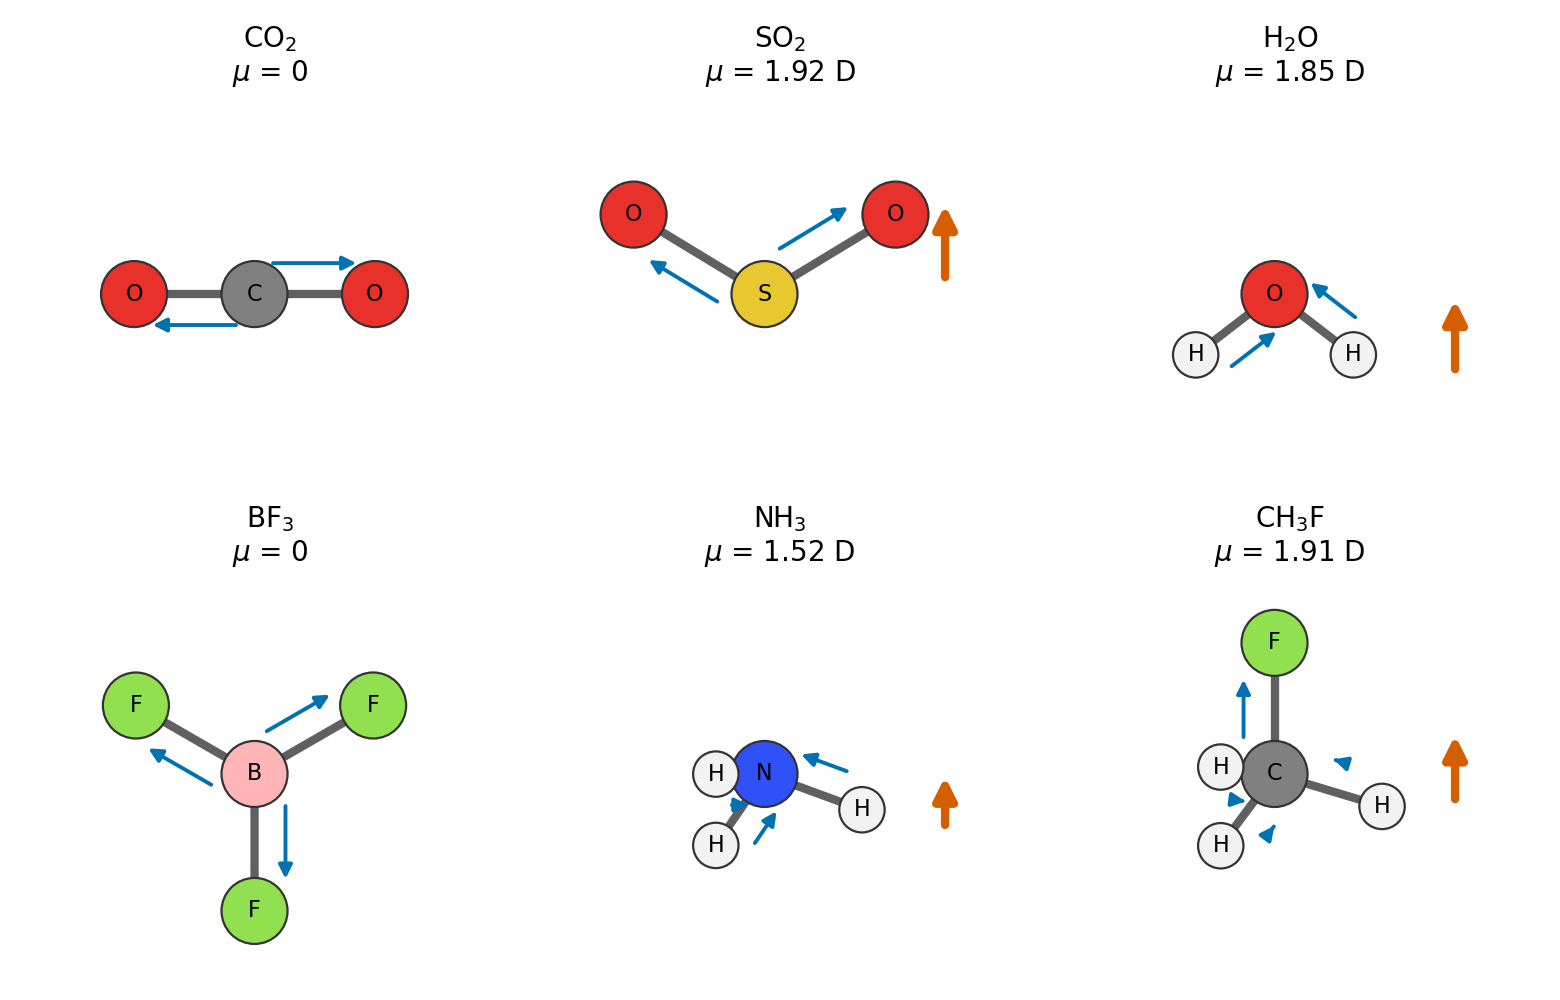
\includegraphics[width=0.95\linewidth]{dipoles/bond-dipoles.ecce-9.5.3-dev.png}
	\caption{Bond dipoles (thin blue arrows, one beside each bond) and the dipole moment of the whole molecule (thick orange arrow, drawn beside the molecule) of six of the molecules of table~\ref{tab:dp}, all pointing towards the negative end. Each bond dipole is the charge of its outer atom times the bond, from the stored atomic charges; the molecular dipole is the calculated dipole moment, at the same scale. \chem{NH3} and \chem{CH3F} are seen from a little above, so that all their atoms show. Drawn from the stored ECCE results.}
	\label{fig:dp-arrows}
\end{figure}

Figure~\ref{fig:dp-arrows} shows the bond dipoles of \chem{CO2} pointing away from each other along one line and those of \chem{BF3} pointing to the corners of a triangle, while those of \chem{SO2}, \chem{H2O}, \chem{NH3} and \chem{CH3F} all lean towards one side of the molecule. This is because the arrows add head to tail: two equal arrows in opposite directions, or three at \ang{120}, end where they started, while arrows that share a direction leave a sum. Hence the thick arrow appears only on the bent and pyramidal molecules and on \chem{CH3F}, whose one strong C--F bond dipole is not balanced by the three weak C--H ones.

\begin{figure}[htbp]
	\centering
	\begin{tabular}{ccc}
		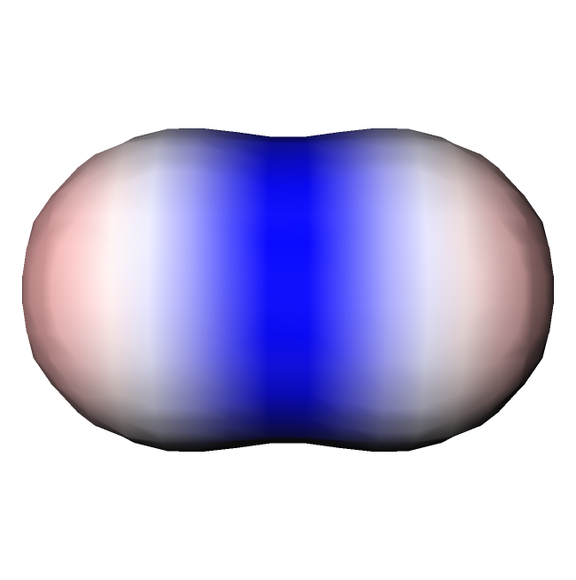
\includegraphics[height=2.6cm]{dipoles/co2-esp.ecce-9.5.3-dev.png} &
		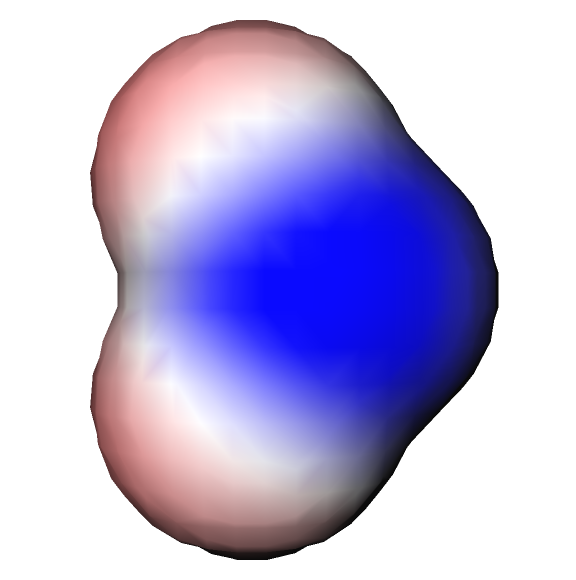
\includegraphics[height=2.6cm]{dipoles/so2-esp.ecce-9.5.3-dev.png} &
		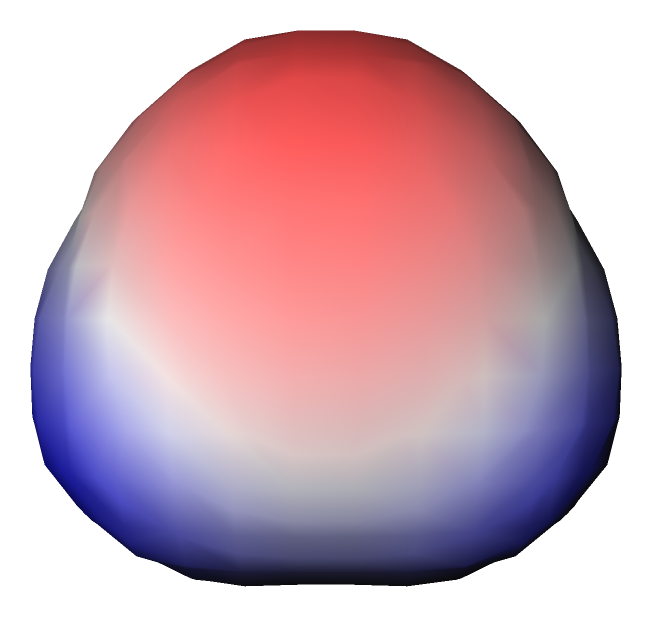
\includegraphics[height=2.6cm]{dipoles/h2o-esp.ecce-9.5.3-dev.png} \\
		\chem{CO2} & \chem{SO2} & \chem{H2O} \\
	\end{tabular}
	\caption{The electric potential on a surface of constant electron density (\menu{ESP on Density} in the \menu{MOs} panel), red negative and blue positive, each picture on its own colour scale (\menu{ESP range: Auto}). \chem{CO2}: the O atoms at the left and right ends, C in the middle. \chem{SO2}: the two O atoms on the left, S on the right. \chem{H2O}: O at the top, the two H atoms at the lower corners.}
	\label{fig:dp-esp}
\end{figure}

Figure~\ref{fig:dp-esp} shows where the charge sits on the outside of each molecule. \chem{CO2} is red at both ends and blue round the middle, symmetric front to back, while \chem{SO2} and \chem{H2O} are red on one side and blue on the other, because a straight molecule puts its negative oxygen atoms at the two ends and a bent one puts them on the same side. Hence a molecule with one red side and one blue side has a dipole moment, and a molecule whose colours are arranged symmetrically has none, which a class can judge from the picture before reading the number.

\section{Adding bond dipoles}
For a bent molecule with two equal bonds the addition can be done on the board. Each bond dipole $\mu_\mathrm{b}$ points along its bond; the components across the molecule cancel and the components along the axis add, so $\mu = 2\mu_\mathrm{b}\cos(\theta/2)$, where $\theta$ is the bond angle. With the calculated values, water ($\mu = 1.85$~D, $\theta = \ang{104.7}$) has a bond dipole of 1.52~D per O--H bond, and \chem{SO2} ($\mu = 1.92$~D, $\theta = \ang{117.5}$) one of 1.85~D per S=O bond. This shows that the bond dipoles of the two molecules are of a similar size, because both bonds join an electronegative atom to a less electronegative one. Hence the angle decides most of the difference between bent and straight molecules: the factor $\cos(\theta/2)$ is 0.61 at \ang{104.7}, 0.52 at \ang{117.5}, and at \ang{180}, the angle of \chem{CO2}, it is zero.
\index{Bond dipole!addition}

The calculated dipole moments of \chem{H2O}, \chem{NH3} and \chem{CH3F} are within 3\,\% of the measured ones; that of \chem{SO2} is 18\,\% too large, so in the calculated column \chem{SO2} comes out as the most polar of the four, while measured it is third. The zeros of the symmetric molecules and the contrast between \chem{CO2} and \chem{SO2} hold exactly in both columns; to rank the four polar molecules, use the measured one.

\section{In class}
Show \chem{CO2} and \chem{SO2} side by side with their charges switched on or their ESP surfaces drawn, ask whether each molecule is polar, and then show the dipole moments. Draw the two bond dipoles as arrows on each molecule; the class can see that the arrows of \chem{CO2} point away from each other along one line and those of \chem{SO2} add up.

\section{History}
Debye introduced the permanent dipole moment of a molecule in 1912 to explain how the dielectric constant of a substance depends on temperature \cite{debye1912}, and collected the theory and the measured values in his book \emph{Polar Molecules} of 1929 \cite{debye1929}.
\index{Debye, Peter}

\chapter{Electron domains and hybridisation}
\label{ch:t-hybridisation}
\XXX[to be written: what the orbitals of methane, ethene and ethyne look like, and what hybridisation describes]

\chapter{The chemical bond in \chem{H2}}
\label{ch:t-h2-bond}
\XXX[to be written: the potential curve, bond length and dissociation energy; restricted and unrestricted at long distance]

\chapter{Bonds, antibonds and bond order}
\label{ch:t-bond-order}
\index{Bond order}
\index{Antibonding orbital}
\index{Hydrogen molecule}\index{Helium dimer}
\eccexample{Examples > General Chemistry > Molecular orbitals of diatomics}

Molecular orbital theory explains why two hydrogen atoms form a molecule and two helium atoms do not with one rule: electrons in a bonding orbital hold the atoms together, electrons in an antibonding orbital push them apart, and the bond order is half the difference. This chapter gives the teacher four molecules that make the rule concrete, \chem{H2+}, \chem{H2}, \chem{He2+} and \chem{He2}, with bond orders \textonehalf, 1, \textonehalf{} and 0, and shows a class that the bond order predicts which bonds are shortest and stiffest, and that \chem{He2} has no bond at all.

\section*{This requires}
Nothing beyond ECCE: the calculations are in the General Chemistry example set.

\section{The calculations}
The topic \menu{Molecular orbitals of diatomics} holds \emph{H2\_cation}, \emph{H2}, \emph{He2\_cation} and \emph{He2}. The first three are optimised structures with their vibrational frequencies. \emph{He2} cannot be optimised, because the two atoms do not bind; it is a single calculation with the atoms held \SI{3.0}{\angstrom} apart.

\section{Procedure}
\begin{enumerate}
	\item In the Organizer, choose \menu{File > Open Example Calculations}, pick \menu{General Chemistry} and click \menu{OK}.
	\item Open \emph{H2} in the Viewer and choose \menu{Properties > Orbitals > MOs}. Note which orbitals are occupied and draw the lowest occupied and the lowest empty orbital with \menu{Compute}.
	\item With \menu{Measure} (Chapter~\ref{ch:first-calculation}), measure the H--H distance, and open \menu{Properties > Vibrational spectra > Vibrational Frequencies} for the stretching frequency.
	\item Repeat for \emph{H2\_cation}, \emph{He2\_cation} and \emph{He2} (\emph{He2} has no frequencies).
\end{enumerate}
\index{MOs panel}

\section{Bond order}
Two 1s orbitals combine into two molecular orbitals: $\sigma$, with the electron density gathered between the nuclei, and $\sigma^*$, with a node half way between them. Filling the orbitals from the bottom gives table~\ref{tab:bo}: \chem{H2+} has one electron in $\sigma$, \chem{H2} two, \chem{He2+} two in $\sigma$ and one in $\sigma^*$, and \chem{He2} two in each. The bond order is (bonding electrons $-$ antibonding electrons)/2.

\begin{figure}[htbp]
	\centering
	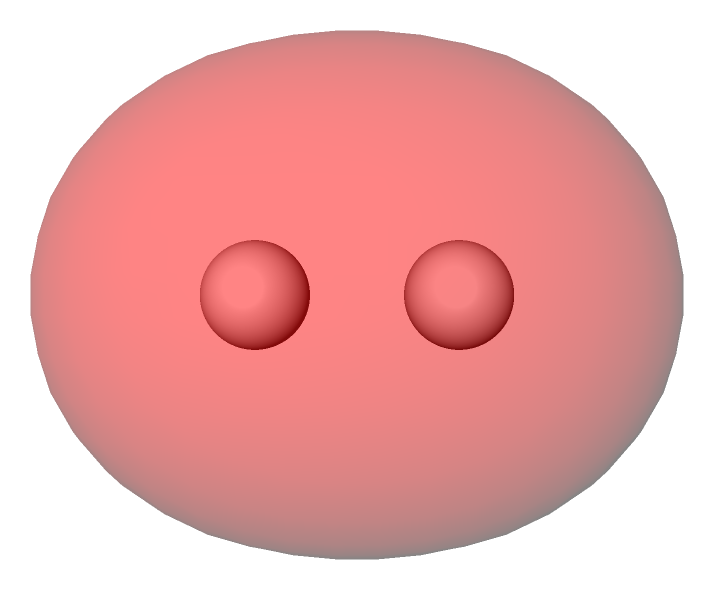
\includegraphics[width=0.3\linewidth]{bond-order/h2-sigma.ecce-9.5.3-dev.png}\hspace{4mm}
	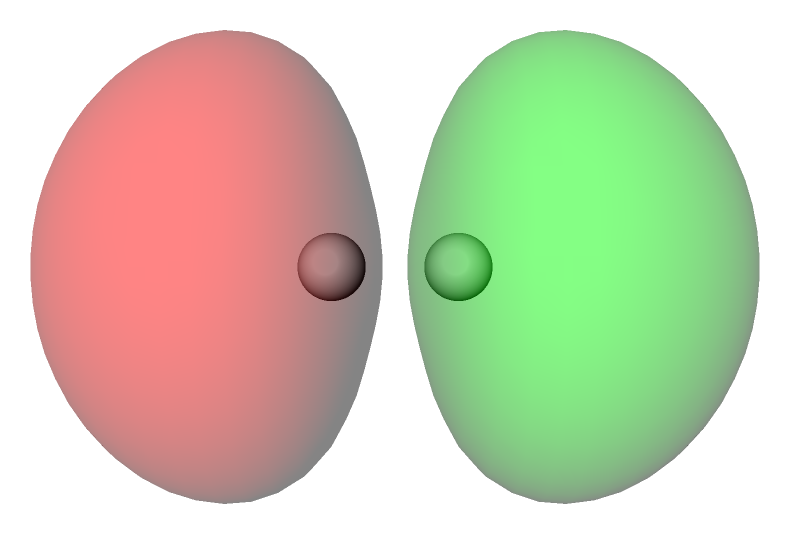
\includegraphics[width=0.3\linewidth]{bond-order/h2-sigmastar.ecce-9.5.3-dev.png}\\[3mm]
	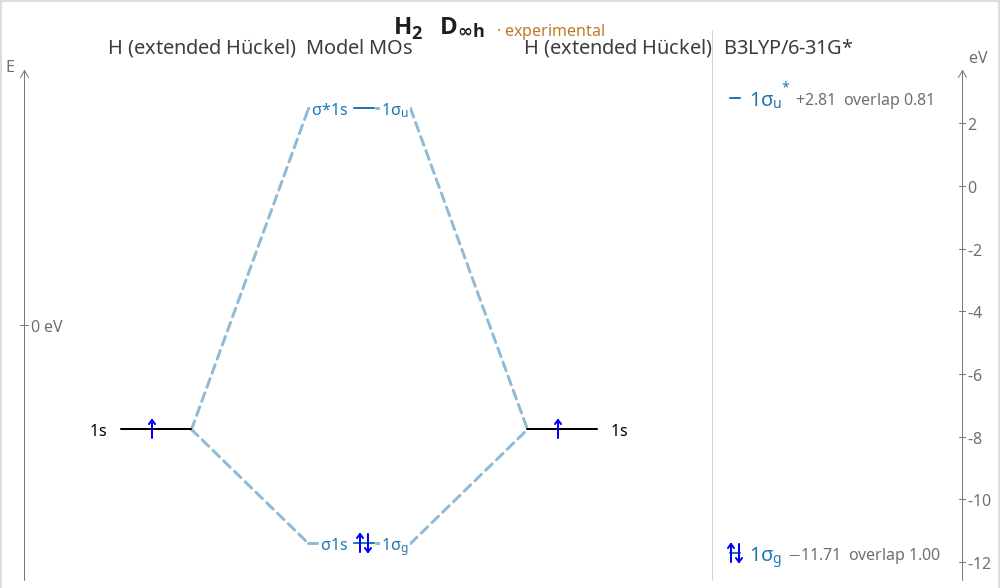
\includegraphics[width=0.75\linewidth]{bond-order/h2-diagram.ecce-9.5.3-dev.png}
	\caption{Top: the bonding $\sigma$ orbital (left) and the empty antibonding $\sigma^*$ orbital (right) of \chem{H2}, drawn in the \menu{MOs} panel; the two colours are the two signs of the orbital. Bottom: the MO diagram of \chem{H2} (\menu{Properties > Orbitals > MO Diagram}): the 1s levels of the two atoms on the left and right, the $\sigma$ and $\sigma^*$ levels between them, and on the far right the levels of the calculation with their energies in eV.}
	\label{fig:bo-h2}
\end{figure}

Figure~\ref{fig:bo-h2} shows that the $\sigma$ orbital is one surface around both nuclei, while $\sigma^*$ is cut in two by an empty plane between them, because in $\sigma$ the two 1s orbitals add and in $\sigma^*$ they cancel half way between the atoms. Hence the electrons in $\sigma$ sit between the nuclei and pull them together, and electrons in $\sigma^*$ sit outside and do not; in the diagram this is the $\sigma$ level below the two 1s levels and the $\sigma^*$ level above them. Each pair of electrons in $\sigma$ is one bond, and each electron in $\sigma^*$ undoes the effect of one in $\sigma$, which is what the bond order counts.

\begin{table}[htbp]
	\centering
	\caption{Electrons in the bonding and antibonding orbitals, bond order, calculated bond length and stretching frequency of the four molecules. The frequency is in wavenumbers (cm$^{-1}$): the higher it is, the stiffer the bond. From the stored ECCE calculations. Measured \cite{nistwebbook}: \chem{H2} \SI{0.741}{\angstrom}; \chem{H2+} \SI{1.052}{\angstrom} and \SI{2322}{cm^{-1}}.}
	\label{tab:bo}
	\begin{tabular}{lccccr}
		\toprule
		Molecule & $\sigma$ & $\sigma^*$ & bond order & bond length (\AA) & frequency (cm$^{-1}$) \\
		\midrule
		\chem{H2}  & 2 & 0 & 1 & 0.743 & 4449 \\
		\chem{H2+} & 1 & 0 & \textonehalf & 1.057 & 2334 \\
		\chem{He2+} & 2 & 1 & \textonehalf & 1.075 & 1746 \\
		\chem{He2} & 2 & 2 & 0 & no bond & -- \\
		\bottomrule
	\end{tabular}
\end{table}

The table shows that \chem{H2}, with bond order 1, has by far the shortest bond, and that the two molecules with bond order \textonehalf{} have bonds about 1.4 times as long, \SI{1.06}{\angstrom} and \SI{1.08}{\angstrom} against \SI{0.74}{\angstrom}. \chem{H2+}, made of the same atoms as \chem{H2}, also vibrates at about half the frequency, so its bond is much softer. This is because each electron in $\sigma$ adds to the glue between the nuclei, and \chem{H2+} has only one such electron, while \chem{He2+} has two but loses most of their effect to the third electron in $\sigma^*$. Hence the bond order, a number worked out by counting, predicts the order of bond lengths and bond strengths without any further calculation.
\index{Bond order!and bond length}

\section{Why \chem{He2} does not exist}
In \chem{He2} the two bonding and two antibonding electrons cancel, and at \SI{3.0}{\angstrom} the $\sigma$ and $\sigma^*$ orbitals lie at $-17.63$ and $-17.54$~eV, almost the same energy (eV, electronvolt, is the energy unit of the MO panel). This shows that the two atoms do not interact at this distance, because orbitals that do not overlap neither lower nor raise each other's energy. Hence there is nothing to gain by moving the atoms closer: bringing them together would lower $\sigma$ but raise $\sigma^*$ by more, and with both full the pair is pushed apart. Helium is a monatomic gas for this reason, while removing one electron, as in \chem{He2+}, leaves bond order \textonehalf{} and a real bond.
\index{Helium dimer!no bond}

\section{In class}
Draw the $\sigma$ and $\sigma^*$ orbitals of \chem{H2} once, then fill in the electrons for the four molecules on the board and let the class predict the order of bond lengths before showing table~\ref{tab:bo}.

\section{History}
Pauling explained the bond of \chem{He2+} in 1933 as a bond held by three electrons \cite{pauling1933}, the case of bond order \textonehalf{} in table~\ref{tab:bo}.
\index{Pauling, Linus}

\chapter{Homonuclear diatomics of the second period}
\label{ch:t-diatomics}
\index{Diatomic molecules}
\index{Molecular orbital diagram}
\index{s--p mixing}
\index{Oxygen!paramagnetism}
\eccexample{Examples > General Chemistry > Molecular orbitals of diatomics}

The molecular orbital diagram of the second-period diatomics is where most students first use MO theory for something a Lewis structure cannot do. This chapter gives the teacher stored calculations of \chem{Li2}, \chem{N2}, \chem{O2} and \chem{F2} for three points of that diagram: the bond order from the diagram predicts the bond lengths and stiffnesses, the order of the $\sigma$ and $\pi$ orbitals made from 2p switches between \chem{N2} and \chem{F2}, and \chem{O2} has two unpaired electrons, which is why liquid oxygen is drawn to a magnet.

\section*{This requires}
Nothing beyond ECCE: the calculations are in the General Chemistry example set.

\section{The calculations}
The topic \menu{Molecular orbitals of diatomics} holds \emph{Li2}, \emph{N2}, \emph{O2} and \emph{F2}, each optimised in the gas phase, with its vibrational frequency. \emph{O2} was calculated with two unpaired electrons, the ground state of the molecule. Orbital energies are in electronvolts (eV); the more negative the energy, the more tightly the orbital holds its electrons.
\XXX[\chem{B2} and \chem{C2} are not in the example set; add them (B$_2$ with two unpaired electrons) to show the consequence of the switched orbital order on the left of the period.]

\section{Procedure}
\begin{enumerate}
	\item In the Organizer, choose \menu{File > Open Example Calculations}, pick \menu{General Chemistry} and click \menu{OK}.
	\item Open \emph{N2} in the Viewer and choose \menu{Properties > Orbitals > MOs}. Draw the highest occupied orbital and the two below it with \menu{Compute}: one is a $\sigma$ orbital along the axis, the other two a pair of $\pi$ orbitals with the same energy.
	\item Repeat for \emph{F2}.
	\item Open \emph{O2} and look at the occupation of the two highest occupied orbitals, the $\pi^*$ pair.
	\item In each molecule, measure the bond length with \menu{Measure} (Chapter~\ref{ch:first-calculation}) and open \menu{Properties > Vibrational spectra > Vibrational Frequencies}.
\end{enumerate}
\index{MOs panel}

\section{Bond order, length and stiffness}
Filling the MO diagram gives bond orders of 1 for \chem{Li2}, 3 for \chem{N2}, 2 for \chem{O2} and 1 for \chem{F2}. Table~\ref{tab:da} shows that from \chem{N2} to \chem{F2} the bond gets longer and softer as the bond order falls, because each pair of electrons added to the antibonding $\pi^*$ orbitals cancels the effect of one bonding pair. Hence the MO diagram predicts the order of the bonds in this series, and the measured bond lengths follow the calculated ones to within \SI{0.01}{\angstrom}. \chem{Li2} has bond order 1 like \chem{F2}, but its bond is twice as long and much softer, because it is held by two 2s electrons far from two small, tightly bound cores.

\begin{table}[htbp]
	\centering
	\caption{Bond order, calculated and measured bond length and calculated stretching frequency of four second-period diatomics. The frequency is in wavenumbers (cm$^{-1}$): the higher it is, the stiffer the bond. Calculated values from the stored ECCE calculations; measured bond lengths from the NIST Chemistry WebBook \cite{nistwebbook}.}
	\label{tab:da}
	\begin{tabular}{lcrrr}
		\toprule
		Molecule & bond order & $R$ calc.\ (\AA) & $R$ meas.\ (\AA) & frequency (cm$^{-1}$) \\
		\midrule
		\chem{Li2} & 1 & 2.730 &       & 341 \\
		\chem{N2}  & 3 & 1.105 & 1.098 & 2457 \\
		\chem{O2}  & 2 & 1.214 & 1.208 & 1656 \\
		\chem{F2}  & 1 & 1.406 & 1.412 & 1055 \\
		\bottomrule
	\end{tabular}
\end{table}

\section{The switch of $\sigma$ and $\pi$}
The 2p orbitals of the two atoms make one bonding $\sigma$ orbital along the axis and two bonding $\pi$ orbitals across it. In \chem{F2} the $\sigma$ orbital lies below the $\pi$ pair, at $-15.9$~eV against $-14.1$~eV, the order of the simplest MO diagram. In \chem{N2} the order is reversed: the $\sigma$ orbital is the highest occupied orbital, at $-11.5$~eV, above the $\pi$ pair at $-12.5$~eV. The drawn surfaces show why. The $\sigma$ orbital of \chem{F2} is made almost only of 2p (88\,\% p), but that of \chem{N2} has a third of its character from 2s (32\,\% s), with large lobes pointing outward from each atom. This is because in nitrogen the 2s and 2p orbitals are close enough in energy to mix, which pushes this $\sigma$ orbital up, while in fluorine the 2s orbital lies too far below 2p to mix. Hence the left of the period, up to \chem{N2}, uses the diagram with $\sigma$ above $\pi$, and \chem{F2} the one with $\sigma$ below $\pi$. \chem{O2} lies at the switch: its $\sigma$ and $\pi$ orbitals are within \SI{1.4}{eV} of each other and their order is not a clean example either way.
\index{s--p mixing!N$_2$ and F$_2$}

\section{Paramagnetic oxygen}
\chem{O2} has twelve valence electrons, two more than \chem{N2}, and they go into the two $\pi^*$ orbitals, which have the same energy. The MO panel shows each $\pi^*$ orbital holding one electron, and both with the same spin, because two electrons in different orbitals of the same energy repel each other least with parallel spins (Hund's rule). Hence \chem{O2} has two unpaired electrons and is paramagnetic: liquid oxygen poured between the poles of a strong magnet stays there, while liquid nitrogen runs through. The Lewis structure O=O, with all electrons paired, gets the double bond right but cannot explain this; the MO diagram explains both.
\index{Oxygen!unpaired electrons}

\section{In class}
Draw the highest occupied orbital of \chem{N2} and the $\sigma$ orbital of \chem{F2} side by side: the extra outward lobes of the \chem{N2} orbital show the 2s mixing that moves it up. Then show the two singly occupied $\pi^*$ orbitals of \chem{O2} together with the liquid-oxygen demonstration, or a video of it.

\section{History}
Lennard-Jones built the molecular orbitals of the second-period diatomics from combinations of atomic orbitals in 1929 and explained with them the paramagnetism of \chem{O2}, which the electron-pair bond of Lewis could not \cite{lennardjones1929}.
\index{Lennard-Jones, John}

\chapter{Polarised bonds and non-bonding orbitals}
\label{ch:t-polarised-bonds}
\XXX[to be written: HF, CO and LiH: unequal sharing in the orbitals]

\chapter{Molecular orbital diagrams from symmetry}
\label{ch:t-symmetry-mos}
\XXX[to be written: H2O, NH3, BH3: orbitals of the ligands combined by symmetry]

\chapter{Methane: canonical and localised orbitals}
\label{ch:t-methane-orbitals}
\XXX[to be written: one orbital at -25 eV and three at -14 eV, and four equal localised bonds from the same density]

\chapter{Benzene and aromaticity}
\label{ch:t-aromaticity}
\XXX[to be written: delocalised pi orbitals, equal bonds, and the stabilisation]

\chapter{Colour from conjugation}
\label{ch:t-conjugation-colour}
\XXX[to be written: longer conjugated chains absorb at longer wavelengths: the polyenes]

\chapter{Vibrational spectra from symmetry}
\label{ch:t-vibrations-symmetry}
\XXX[to be written: which modes are IR or Raman active, and why]

\chapter{Greenhouse gases}
\label{ch:t-greenhouse}
\XXX[to be written: the IR-active bending and stretching modes of CO2, H2O and CH4 against N2 and O2]

\chapter{Crystal and ligand field: colours of complexes}
\label{ch:t-ligand-field}
\XXX[to be written: d-orbital splitting in octahedral complexes, and the colour it gives]

\chapter{Maxwell's distribution of speeds}
\label{ch:t-maxwell}
\XXX[to be written: speeds of gas molecules from a molecular dynamics run, against the formula]

\chapter{Gases, liquids and solids}
\label{ch:t-phases}
\XXX[to be written: the same molecules in three phases from molecular dynamics: water vapour, liquid and ice]

\chapter{Ion-dipole interactions}
\label{ch:t-ion-dipole}
\XXX[to be written: Na+ with water: the energy and the orientation of the molecules]

\chapter{The hydrogen bond: the water dimer}
\label{sec:hydrogen-bond}
\index{Hydrogen bond}
\index{Water dimer}
\index{Intermolecular interactions}
\checkedwith{9.5.3-dev}{6dd630422}
\eccexample{Examples > General Chemistry > Intermolecular interactions}
\helppage{density-map}

\helppage{electron-density-views}

The hydrogen bond is usually drawn as a dotted line between a hydrogen atom and an oxygen or nitrogen atom of another molecule. This chapter gives the teacher pictures and numbers to show a class what that line stands for, all taken from two stored calculations of the General Chemistry example set: the water dimer, the smallest case of the bond, and the single water molecule. Each section takes one sign of the bond that students meet in a course, namely the energy that holds the pair together, the short distance between the molecules and the longer O--H bond of the donor, the lower and stronger O--H stretch in the infrared spectrum, and the electron density between the molecules, and names the ECCE panel that shows it and the chemical point it makes.

\section*{This requires}
Nothing beyond ECCE: the calculations are in the General Chemistry example set.

\section{Background}
This section gives the chemistry that the pictures in the rest of the chapter are read against. In O--H$\cdots$O the donor O--H group gives up a little electron density to the region between H and the acceptor oxygen. The attraction is mostly electrostatic: the positive end of one O--H dipole points at the negative region of the other molecule. In the water dimer the donor O--H points almost straight at the acceptor oxygen, and the acceptor's two hydrogens lie out of the plane of the bond.

A hydrogen bond between neutral molecules is far weaker than a covalent bond and several times stronger than the attraction between molecules of similar size without one. That is enough to give water its high boiling point and ice its open structure.

\section{The calculation}
The topic \menu{Intermolecular interactions} has two calculations made for this chapter, the water dimer \emph{h2o\_dimer} and the single molecule \emph{h2o\_monomer}. Both were optimised and their vibrations calculated with the same method, so their energies, structures and spectra can be compared directly.

\section{Procedure}
The steps show where in ECCE each number and picture of this chapter comes from; the sections that follow take them in the same order.
\begin{enumerate}
	\item In the Organizer, choose \menu{File > Open Example Calculations}, pick \menu{General Chemistry} and click \menu{OK}.
	\item In \menu{Examples > Intermolecular interactions}, select \emph{h2o\_dimer} and \emph{h2o\_monomer} and compare their total energies in the Organizer's table, or with \menu{Tools > Energy Calculator...}: dimer minus twice the monomer.
	\item Open \emph{h2o\_dimer} in the Viewer. With \menu{Measure} (Chapter~\ref{ch:first-calculation}), measure the distances O1--O4, H2--O4 and O1--H2, and the angle O1--H2--O4. Measure O--H in \emph{h2o\_monomer} too.
	\item Open \menu{Properties > Vibrational spectra > Vibrational Frequencies} in both and compare the O--H stretches above 3000~cm$^{-1}$, with their IR intensities.
	\item In the dimer, click \menu{Density Map}, choose the plane \menu{Through three atoms A, B, C} with O1, H2 and O4, and \menu{Show: Total density}. Click \menu{Density Profile} for the same density along the line from O1 to O4.
	\item Open \menu{Properties > Orbitals > Surfaces} and choose \menu{NCI}.
\end{enumerate}
\index{Energy Calculator}\index{Measure}\index{NCI}

\section{Interaction energy}
The first question for a class is whether the two molecules hold together at all, and how strongly. The dimer is \SI{26}{kJ.mol^{-1}} lower in energy than two separate molecules ($-152.862864$ against $2\times-76.426490$~hartree, the unit in which ECCE lists these energies; one hartree is \SI{2625.5}{kJ.mol^{-1}}). That is the energy it takes to pull the pair apart, the strength of this one hydrogen bond. It is about ten times $RT$ at room temperature (\SI{2.5}{kJ.mol^{-1}}), the typical energy that molecules exchange in collisions, because the positive end of the donor's O--H dipole sits right against the negative region of the acceptor oxygen. Hence a hydrogen bond survives many collisions before it breaks, which is why the molecules of liquid water stay held by their neighbours, while the bond is still weak enough to break and form again all the time.

\section{Geometry}
The bond also shows in the structure, measured with \menu{Measure}. O1--O4 is \SI{2.90}{\angstrom} and H2--O4 \SI{1.93}{\angstrom}, well inside the sum of the van der Waals radii of H and O (about \SI{2.7}{\angstrom}), the distance at which an H atom and an O atom of two molecules touch without any bond between them. The angle O1--H2--O4 is \ang{172.6}, nearly linear. The donor's O1--H2 bond is \SI{0.971}{\angstrom}, \SI{0.008}{\angstrom} longer than O--H in the single molecule (\SI{0.963}{\angstrom}).

The short H2--O4 distance shows that the molecules are pulled closer together than two molecules merely in contact, because H2 is attracted to O4, and the longer O1--H2 shows that this attraction weakens the donor's own bond, because it draws some of the density of that bond towards O4. Hence the hydrogen bond can be seen in the structure alone, and the weaker donor bond is what the infrared spectrum picks up next.

\section{Infrared spectrum}
The infrared spectrum is where a hydrogen bond is most often seen in a laboratory, and the \menu{Vibrational Frequencies} panel shows the calculated spectrum. The single molecule has its two O--H stretches at 3782 and 3888~cm$^{-1}$. In the dimer the stretch of the bonded O--H is at 3668~cm$^{-1}$, \SI{114}{cm^{-1}} lower, with an IR intensity of 315~km/mol against 4 and 44~km/mol in the single molecule. The intensity says how strongly a band absorbs infrared light, so the band of the bonded O--H is seven times as strong as the stronger O--H band of the single molecule. The other three stretches of the dimer, at 3780, 3858 and 3880~cm$^{-1}$, stay close to those of the free molecule.

The lower frequency follows from the structure, since the longer, weaker O1--H2 bond vibrates more slowly, and only the stretch of the bonded O--H shifts, which shows that the effect is confined to the bond that points at the acceptor. A low and strong O--H band, broad in a measured spectrum, is how a hydrogen bond is recognised in the laboratory.
\index{Infrared spectrum!hydrogen bond}\index{Red shift}

\section{Electron density}
The \menu{Density Map} and \menu{Density Profile} panels show where the electrons are between the two molecules, which is the way to ask what the dotted line of the textbook stands for. In the plane of the bond (figure~\ref{fig:hb-density}) the inner contours of the total density close around each molecule separately, and only the outer, low levels enclose both, with a narrow waist between H2 and O4, so the dimer remains two molecules held close together.

\begin{figure}[htbp]
	\centering
	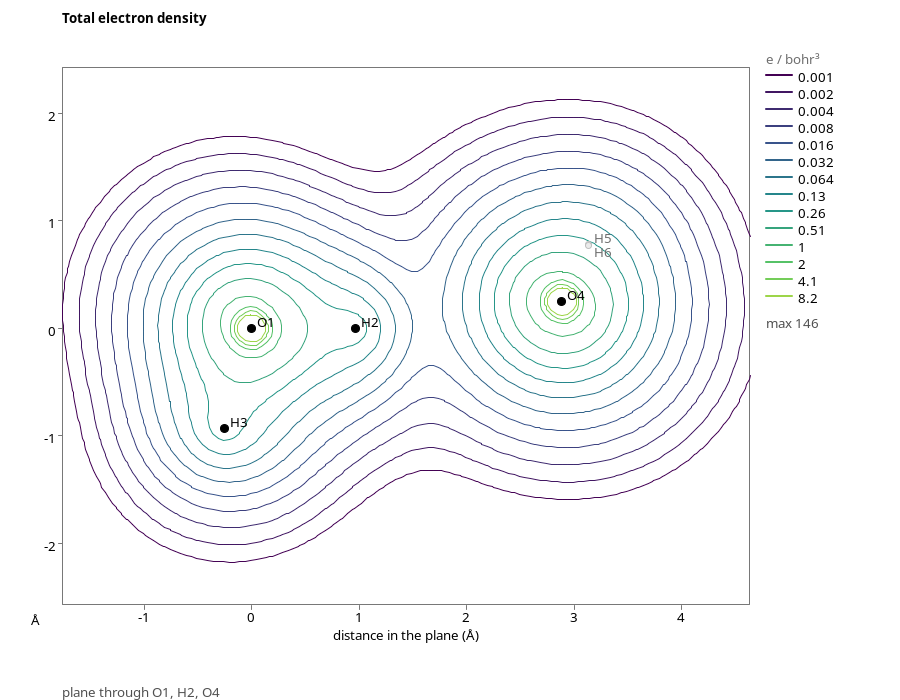
\includegraphics[width=0.8\linewidth]{hydrogen-bond/total-density.ecce-9.5.3-dev.png}
	\caption{Total electron density of the water dimer in the plane through O1, H2 and O4 (\menu{Density Map}). The contour levels double from 0.001~e/bohr$^3$ (0.001, 0.002, 0.004, \ldots), so each ring inward has twice the density of the one outside it. Only the outermost rings enclose both molecules.}
	\label{fig:hb-density}
\end{figure}

The \menu{Density Profile} along the line from O1 to O4, which passes almost through H2, puts numbers on the waist of the map (figure~\ref{fig:hb-profile}). The density is in electrons per cubic bohr (one bohr is \SI{0.529}{\angstrom}), on a logarithmic axis where each grid line is ten times the one below. Between H2 and O4 the density falls to a minimum of 0.0255~e/bohr$^3$, 0.66~\AA\ from H2. In the covalent O1--H2 bond it does not fall below 0.34~e/bohr$^3$, about thirteen times as much. The profile shows that the two molecules share very little electron density, because the hydrogen bond is mostly the electrostatic attraction of two separate molecules rather than an electron pair shared between them. Hence it is far weaker than a covalent bond, while the small density between H2 and O4 is still there, and the next view shows what kind of contact it is.
\index{Density Profile!hydrogen bond}

\begin{figure}[htbp]
	\centering
	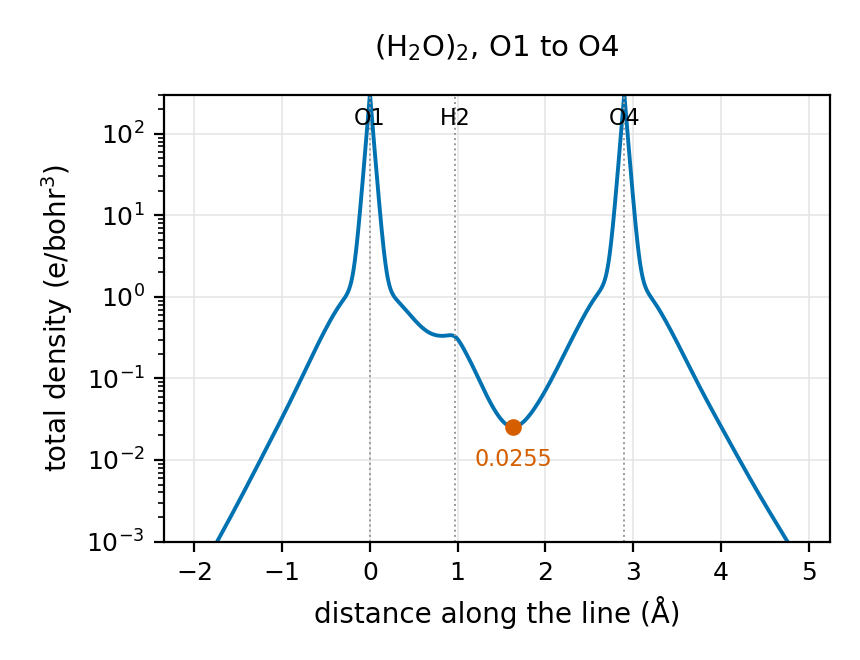
\includegraphics[width=0.6\linewidth]{hydrogen-bond/density-profiles.ecce-9.5.3-dev.png}
	\caption{Total electron density along the line from O1 to O4 of the water dimer (\menu{Density Profile}, logarithmic axis). The dot marks the lowest density between H2 and O4, 0.0255~e/bohr$^3$, about a thirteenth of the lowest density in the covalent O1--H2 bond.}
	\label{fig:hb-profile}
\end{figure}

\section{Non-covalent interactions}
The density map shows that there is a little density between H2 and O4, but not whether it pulls the molecules together or pushes them apart. The \menu{NCI} surface (non-covalent interactions) answers that, and it puts the hydrogen bond in one place in the picture (figure~\ref{fig:hb-nci}). ECCE draws the surface only where the electron density is low and changes slowly, which is true between molecules but not inside the covalent bonds or around the nuclei, so the bonds of each water molecule carry no surface and only the contacts between molecules do. It then colours the surface by the density there, with a sign that tells whether the density is gathered between two atoms or pushed apart: blue for attraction such as a hydrogen bond, green for weak contacts with little density, such as two molecules merely touching, and red for repulsion between atoms crowded too close. The colours run on one fixed scale for every calculation, so a blue surface in one molecule means the same as a blue surface in another.

In the water dimer the only surface is a small disc between H2 and O4, across the line between them, and it is blue. This shows that the density between the two molecules marks an attraction, because it is gathered between H2 and O4 rather than pushed apart. Hence the dotted line of the textbook has a place in the molecule, and the disc is where it crosses from one water molecule to the other.

\begin{figure}[htbp]
	\centering
	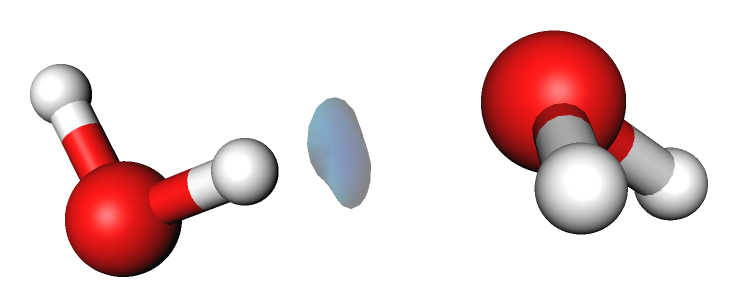
\includegraphics[width=0.6\linewidth]{hydrogen-bond/nci.ecce-9.5.3-dev.png}
	\caption{NCI surface of the water dimer (\menu{Properties > Orbitals > Surfaces}, \menu{NCI}), donor on the left and acceptor on the right. The only surface is the small disc between H2 and O4. Its colour tells the kind of contact on a fixed scale: blue attraction, as in a hydrogen bond; green a weak contact with little density; red repulsion. The disc is blue, an attraction; the surface is drawn partly transparent, which makes the blue look pale on a white background.}
	\label{fig:hb-nci}
\end{figure}

\section{In class}
Show the evidence in the order energy, distance, infrared, density: each is one more piece of evidence for the same bond, and the first three can be measured in a laboratory. The density map is the place to ask what the dotted line in the textbook stands for. It is not a line of electrons; the molecules stay separate, and what the map shows is a small extra amount of density between H and O on top of the overlap of two molecules. The NCI surface then puts the bond in one place, the blue disc between H2 and O4.

\section{History}
For a class, the origin of the idea shows that the hydrogen bond was proposed to explain the properties of water, the same properties the Background starts from. Latimer and Rodebush proposed in 1920 that a hydrogen atom held between two strongly electronegative atoms could bind them, to explain the properties of water and of hydrogen fluoride \cite{latimer1920}. Pauling made the hydrogen bond a part of structural chemistry in the 1930s, and it became central to biochemistry when it was shown to hold the base pairs of DNA and the helices and sheets of proteins together.
\index{Latimer, Wendell}\index{Rodebush, Worth}\index{Pauling, Linus}

\chapter{London dispersion}
\label{ch:t-dispersion}
\index{London dispersion}
\index{Argon dimer}
\index{Intermolecular interactions}
\eccexample{Examples > General Chemistry > Intermolecular interactions}

Two argon atoms carry no charge and no dipole, and their electron shells are closed, yet argon condenses when it is cold enough, so something must hold the atoms together. The attraction is London dispersion: the electron clouds of the two atoms fluctuate, and the fluctuations in one atom are correlated with those in the other, so that the pair is on average a little lower in energy close together than far apart. This chapter gives the teacher one curve, the energy of two argon atoms against their distance, to show a class that this attraction exists, how weak it is next to a hydrogen bond, and why it still matters. The argon dimer is the cleanest case to show, since nothing else contributes.

\section*{This requires}
Nothing beyond ECCE: the calculation is in the General Chemistry example set.

\section{The calculation}
The topic \menu{Intermolecular interactions} holds the argon dimer \emph{ar\_dimer}, optimised in ECCE in the same way as the water dimer of Chapter~\ref{sec:hydrogen-bond}. For the curve of figure~\ref{fig:disp-curve} the Ar--Ar distance was scanned (Chapter~\ref{ch:scans}), from \SI{0.4}{\angstrom} inside the optimised distance out to \SI{10}{\angstrom}. Each point is the energy of the pair relative to two argon atoms calculated separately, in kJ/mol, the energy per mole of pairs; a negative value means that the pair is held together by that much energy.

\section{The curve}
The curve shows how deep the attraction is and how it changes with distance. Its lowest point is at \SI{3.78}{\angstrom}, only \SI{1.2}{kJ.mol^{-1}} below two separate argon atoms (table~\ref{tab:disp-curve}). Spectroscopy of argon dimers in the gas phase puts the bottom of the real well at \SI{3.76}{\angstrom} and \SI{1.19}{kJ.mol^{-1}} (99.2~cm$^{-1}$) below the separate atoms \cite{herman1988}, so the calculated curve has both the position and the depth of the measured one. The two sides of the well are very different: moving the atoms \SI{0.4}{\angstrom} closer than the minimum raises the energy by \SI{1.3}{kJ.mol^{-1}}, more than the whole depth of the well, while moving them \SI{0.4}{\angstrom} apart costs only \SI{0.3}{kJ.mol^{-1}}. The steep inner wall is the repulsion of the two closed shells, which sets in abruptly once they touch, and the shallow outer side is the dispersion attraction, which dies away slowly with distance. Hence the curve shows both halves of the familiar picture of atoms as soft spheres, a hard core with a weak, long attractive tail. Beyond about \SI{8}{\angstrom} the points scatter by a few hundredths of a kJ/mol around zero; that is the numerical precision of the calculation, not a feature of the attraction.

\begin{figure}[htbp]
	\centering
	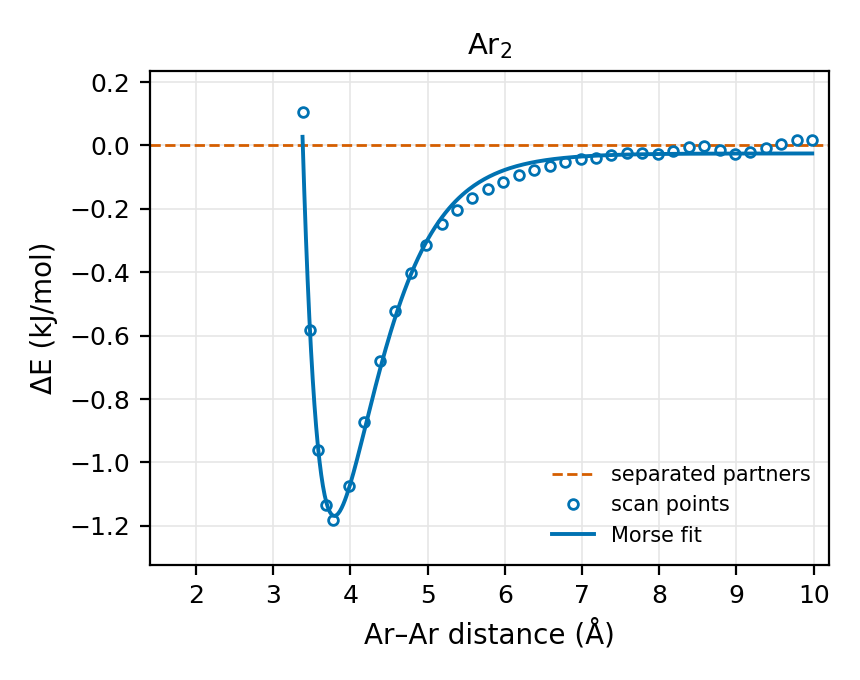
\includegraphics[width=0.6\linewidth]{dispersion/dispersion-curve.ecce-9.5.3-dev.png}
	\caption{Energy of the argon dimer against the Ar--Ar distance, from a relaxed scan in ECCE. Zero (dashed) is two argon atoms calculated separately. Note the energy scale, about twenty times smaller than that of the water dimer in figure~\ref{fig:hb-curve}.}
	\label{fig:disp-curve}
\end{figure}

\begin{table}[htbp]
	\centering
	\caption{The curve of figure~\ref{fig:disp-curve}. $\Delta E_\mathrm{min}$ is the lowest point, at the distance $R_\mathrm{min}$, and $\Delta E(R_\mathrm{max})$ the point at the largest distance $R_\mathrm{max}$, both relative to two separate argon atoms. Energies in kJ/mol.}
	\label{tab:disp-curve}
	\begin{tabular}{rrrr}
		\toprule
		$R_\mathrm{min}$ (\AA) & $\Delta E_\mathrm{min}$ & $\Delta E(R_\mathrm{max})$ & $R_\mathrm{max}$ (\AA) \\
		\midrule
		3.78 & $-1.2$ & 0.0 & 9.98 \\
		\bottomrule
	\end{tabular}
\end{table}

The comparison with the hydrogen bond puts the depth in proportion. The water dimer, scanned in the same way, is \SI{25.9}{kJ.mol^{-1}} deep (Chapter~\ref{sec:hydrogen-bond}), about twenty times deeper than the argon well. At room temperature $RT$, the typical energy that molecules exchange in collisions, is \SI{2.5}{kJ.mol^{-1}}, twice the depth of the argon well, so collisions break an argon pair apart almost as soon as it forms. Hence argon is a gas at room temperature and becomes a liquid only when it is cooled far enough for collisions to be gentle compared with the depth of the well. Argon boils at \SI{87.3}{K} (\SI{-185.9}{\celsius}) \cite{gosman1969}, where $RT$ is \SI{0.73}{kJ.mol^{-1}}, less than the depth of the well.
\index{Relaxed scan!interaction curves}

\section{Non-covalent interactions}
The \menu{NCI} surface (\menu{Properties > Orbitals > Surfaces}, \menu{NCI}), described with the water dimer in Chapter~\ref{sec:hydrogen-bond}, shows the contact between the two argon atoms in the same way. ECCE draws it only where the electron density is low and changes slowly, and colours it on one fixed scale: blue for an attraction with density gathered between two atoms, as in a hydrogen bond, green for a weak contact with very little density, and red for atoms crowded too close. In the argon dimer at its minimum the only surface is a single disc halfway between the two atoms, across the line joining them, and it is green (figure~\ref{fig:disp-nci}).

This figure shows that the two atoms meet in a contact with very little electron density, because green is the colour the fixed scale gives where the density between the atoms is close to zero. Hence we can see that the argon atoms are only touching, held by the weak attraction of the shallow well in figure~\ref{fig:disp-curve}, and not by an attraction with density gathered between them as in a hydrogen bond.
\index{NCI}

\begin{figure}[htbp]
	\centering
	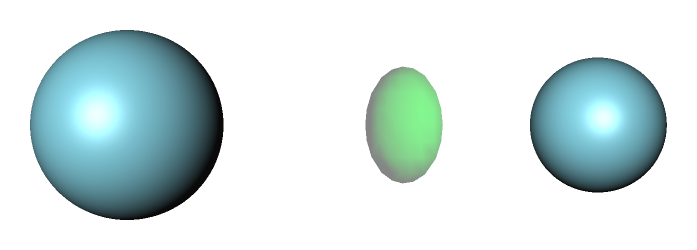
\includegraphics[width=0.6\linewidth]{dispersion/nci.ecce-9.5.3-dev.png}
	\caption{NCI surface of the argon dimer at its minimum (\menu{Properties > Orbitals > Surfaces}, \menu{NCI}). The only surface is the disc halfway between the two atoms. Its colour tells the kind of contact on a fixed scale: blue attraction, as in a hydrogen bond; green a weak contact with little density; red repulsion. The disc is green. The molecule is turned so that the disc shows; the left atom is nearer the viewer and looks larger.}
	\label{fig:disp-nci}
\end{figure}

\section{Three contacts side by side}
The NCI surfaces of three chapters set side by side (figure~\ref{fig:disp-nci-three}) give a class the kinds of contact in one picture: the argon dimer of this chapter, the water dimer of Chapter~\ref{sec:hydrogen-bond} and Na$^+\cdots$H$_2$O of Chapter~\ref{ch:t-ion-dipole}. Each has one disc between the partners. The argon disc is green, while the discs of the hydrogen bond and of the ion--water contact are both pale blue and look much alike, so the colour separates a weak dispersion contact from an attraction with density between the partners, but not a hydrogen bond from an ion--dipole contact; their strengths are told apart by the energies of the curves. None of the three shows red, since at the optimised distance no atoms are pushed together too closely.

This figure shows that dispersion is a different kind of contact from the hydrogen bond and the ion--dipole attraction, because the same fixed colour scale makes the argon disc green and the other two blue. Hence we can see in one picture that argon atoms are held by a weaker kind of contact than the one that holds two water molecules together or a water molecule to a dissolved ion.

\begin{figure}[htbp]
	\centering
	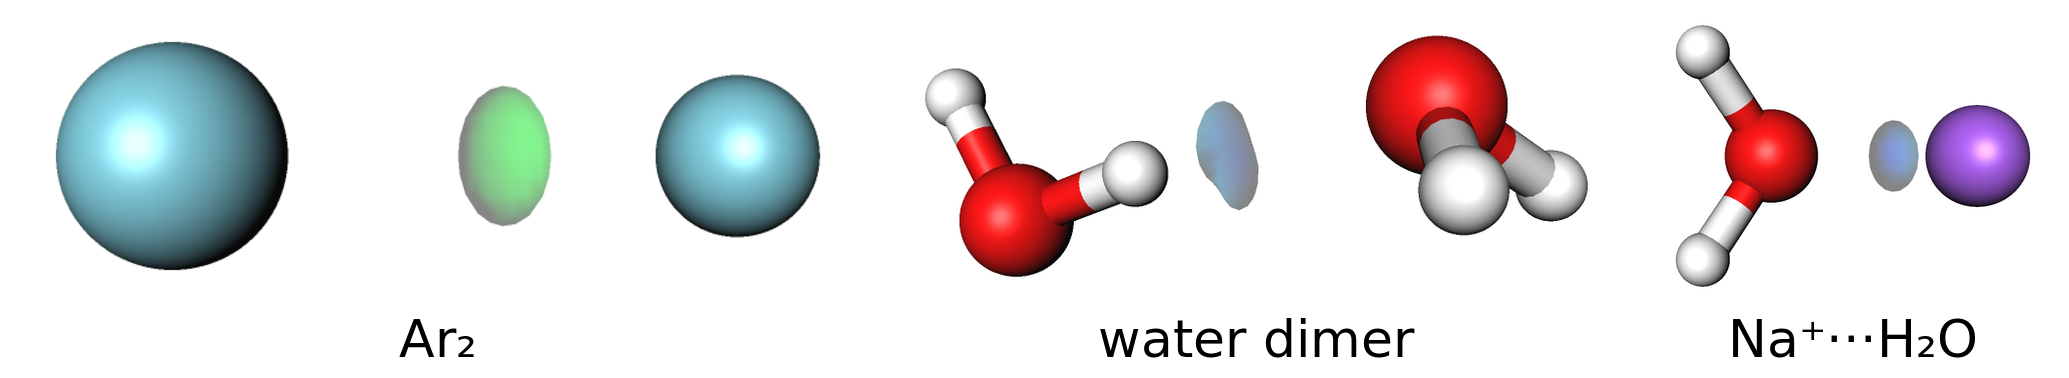
\includegraphics[width=\linewidth]{dispersion/nci-three.ecce-9.5.3-dev.png}
	\caption{NCI surfaces of the argon dimer (left, figure~\ref{fig:disp-nci}), the water dimer (middle, figure~\ref{fig:hb-nci}) and Na$^+\cdots$H$_2$O (right, figure~\ref{fig:id-nci}), each at its optimised structure, on the same fixed colour scale: blue attraction, green a weak contact with little density, red repulsion. The argon disc is green, the other two are blue; the surfaces are drawn partly transparent, which makes the blue look pale on a white background.}
	\label{fig:disp-nci-three}
\end{figure}

\section{In class}
Start with the question why argon, with no charges, no dipoles and full shells, becomes a liquid at all, and then show figure~\ref{fig:disp-curve} with its numbers next to those of the water dimer. Figure~\ref{fig:disp-nci-three} then shows the difference in colour: green for argon, blue for the hydrogen bond and for the ion next to a water molecule. The attraction between two single atoms is weak, but dispersion acts between every pair of atoms in contact, so it adds up for large molecules; this is why the boiling points of the straight-chain alkanes rise with chain length.

\section{History}
Van der Waals gave real gases an attraction between their molecules in his thesis of 1873, as the constant $a$ of his equation of state, without saying where the attraction came from \cite{vanderwaals1873}. Debye in 1920 and Keesom in 1921 traced it to the electric moments of the molecules: a permanent dipole or quadrupole induces a dipole in its neighbour (Debye), and permanent moments that rotate attract each other on average (Keesom) \cite{debye1920,keesom1921}. Neither mechanism applies to atoms of the noble gases, which have no permanent moments, and yet argon condenses. Jones (later Lennard-Jones) fitted an intermolecular potential with an attractive and a repulsive power of the distance to the equation of state of argon in 1924 \cite{jones1924}, and in 1931 settled on the form with $R^{-6}$ attraction and $R^{-12}$ repulsion that carries his name \cite{lennardjones1931}.
\index{van der Waals, Johannes Diderik}\index{Debye, Peter}\index{Keesom, Willem Hendrik}\index{Lennard-Jones, John}

The $R^{-6}$ attraction itself was explained by quantum mechanics. Eisenschitz and London calculated it for two hydrogen atoms in 1930, and London gave the general treatment the same year: the momentary dipoles of the two electron distributions are correlated, which lowers the energy of the pair by an amount that falls off as $R^{-6}$ \cite{eisenschitz1930,london1930}. London called the effect dispersion, after its connection with the optical dispersion of the atoms, and his 1937 paper in the Transactions of the Faraday Society gave the theory in English \cite{london1937}.
\index{London, Fritz}\index{Eisenschitz, Robert}

\chapter{Packing and unit cells}
\label{ch:t-packing}
\XXX[to be written: close packing, unit cells and coordination numbers in metals and salts]

\chapter{Molecular, covalent and layered solids}
\label{ch:t-solids}
\XXX[to be written: ice, dry ice, quartz, diamond and graphite compared]

\chapter{Bragg's law and X-ray diffraction}
\label{ch:t-bragg}
\XXX[to be written: a powder pattern from a crystal, and what the peaks mean]

\chapter{Photograph 51 and the alpha helix}
\label{ch:t-photograph-51}
\XXX[to be written: fibre diffraction patterns of DNA and a helical protein]

\chapter{Reaction energies and activation}
\label{ch:t-reaction-energies}
\XXX[to be written: an SN2 reaction: reaction energy, barrier and the Arrhenius equation]

\chapter{Acids and bases}
\label{ch:t-acids-bases}
\XXX[to be written: proton affinities and the site a proton prefers]

\chapter{Chemical equilibrium}
\label{ch:t-equilibrium}
\XXX[to be written: equilibrium constants from calculated free energies]

\chapter{Hartree-Fock and density functional theory}
\label{ch:t-hf-dft}
\XXX[to be written: what each method leaves out, shown on the same molecule]

\chapter{Basis sets}
\label{ch:t-basis-sets}
\XXX[to be written: how a property converges as the basis set grows]

\chapter{Restricted and unrestricted calculations}
\label{ch:t-restricted-unrestricted}
\XXX[to be written: closed and open shells, and spin contamination]

